\documentclass{msuphddissertation}
\usepackage{amsmath}
\usepackage{amsfonts}
\usepackage{graphicx}
\usepackage{enumitem}
\usepackage{minibox}
\usepackage{color}
\usepackage{tabularx}
\usepackage{siunitx}\sisetup{per-mode=symbol}
\usepackage{listings} 
\usepackage[T1]{fontenc}
\usepackage{xparse}
\usepackage{enumitem}
\setlist[description]{
  font={\bfseries},
  labelsep=0pt,
  labelwidth=\transcriptlen,
  leftmargin=\transcriptlen}
\newlength{\transcriptlen}
\NewDocumentCommand {\setspeaker} { mo } {
  \IfNoValueTF{#2}
  {\expandafter\newcommand\csname#1\endcsname{\item[#1:]}}
  {\expandafter\newcommand\csname#1\endcsname{\item[#2:]}}
  \IfNoValueTF{#2}
  {\settowidth{\transcriptlen}{#1}}
  {\settowidth{\transcriptlen}{#2}}}
\setspeaker{SA}
\setspeaker{SB}
\setspeaker{SC}
\setspeaker{SD}
\setspeaker{TA}
\addtolength{\transcriptlen}{1em}

%
%
%
%
%
%
%
%
%	FRONT MATTER
%
%
%
%
%
%
%
%

\author{Michael J. Obsniuk}
\title{Identifying Computational Practices in Introductory Physics}
\unit{Physics --- Doctor of Philosophy}

\begin{document}

\maketitlepage

\begin{abstract}
Introduction, Background, Context, Motivation, Analysis, Discussion, Conclusion.
\end{abstract}

\TOC
\LOT
\LOF

\newpage
\pagenumbering{arabic}
\begin{doublespace}

%
%
%
%
%
%
%
%
%	INTRODUCTION
%
%
%
%
%
%
%
%

\chapter{Introduction}\label{CH1:Introduction}

Since the advent of relatively inexpensive and powerful computers, researchers have been interested in their use as both professional and pedagogical tools.  Their ability to quickly and precisely perform numerical calculation makes them well suited for modeling and solving modern problems in the STEM fields.  Similarly, their ability to easily generate meaningful visualizations makes them well suited for the communication of scientific information.  For these reasons, computation is indispensible in modern scientific pursuits.

Computation, or the use of computers to analyze complicated problems, continues to grow in many fields, from mathematics to biology.  Given its utility in these professional domains, the task of effectively training students in computation has risen to the forefront of education research.  This task has been shown to involve many challenges, as there are many and varied skills and pieces of knowledge that students must develop a mastery of in order to effectively utilize computation.  Still, the desire to integrate computation into the STEM curriculum is stronger than ever.

While using computation to solve complex physics and engineering problems, practitioners often engage in various computational practices.  Computational practices can be defined as a synthesis of computational knowledge and computational skill -- highlighting the importance of being able to put theoretical ideas to practical work.  Although knowledge and skill alone are important, being able to combine the two into an effective \textit{practice} is even more so.  Although attempts have been made to define computational practices broadly, they are still lacking clear and precise definition within many particular domains (e.g., computational physics). Accordingly, this thesis focuses on identifying the common computational physics practices that students engage in while solving realistic physics and engineering problems.

There are a number of reasons for focusing on computational physics and its associated computational practices.  Perhaps most important is that there is a high demand for computational skills in the workplace for physics graduates \cite{AAPT2016}.  Being able to effectively prepare students requires in-depth research to develop best practices.  Modern physics curricula should reflect the modern practices of professional physicists, and computation is often seen as just as important as theory and experiment.  For this reason, $\SI{51}{\percent}$ of faculty from physics departments call for more computation in the curriculum \cite{Chonacky2008}.

Additionally, it is believed that students of computational physics gain a deeper understanding of the physical concepts \cite{Chabay2008,Kohlmyer2005}.  Visual packages such as VPython or Glowscript \cite{Sherer2000} allow novice programmers to create stunning three-dimensional visualizations that allow them to more easily interact with the fundamental concepts.

Further, computation allows for the analysis of realistic problems that have no closed-form solution.  Its ability to numerically integrate supports a more exploratory approach to analyzing physical systems and learning physics.  That is, the repeated application of Newton's second law allows for a more general analysis.  This more exploratory approach is thought to encourage students to construct more realistic and accurate computational models through computational thinking \cite{AAPT2016}.

Finally, computational thinking is a term that has become increasingly popular since its introduction in the early 1980s.  This term, although frequently used today, is difficult to concisely explain given its many and varied definitions.  Even within the fields of education and computer science, many different viewpoints exist on the topic, and the corresponding definitions are just as varied \cite{Grover2013}.  However, many of these definitions share one fundamental characteristic: solving complex problems through abstraction and analytic thinking with the aid of computer algorithms, which is precisely the type of thinking that this thesis explores.

Computational thinking is so highly valued by the modern enterprise of science education that the Next Generation Science Standards (NGSS) laid out a framework for identifying computational thinking in K-12 settings.  As early as the fifth grade students are expected to be able to think computationally.  They describe computational thinking, at this level, in terms of analyzing data and comparing approaches.  By the time students reach middle school, computational thinking advances to analyzing large data sets and generating explanations.  Finally, in high school, computational thinking expands to constructing computational models and using them to answer questions \cite{NGSS2012}.  Clearly, computational thinking is a complicated concept which requires substantial explanation.

Experts in the field still have a ways to go when it comes to clearly defining computational thinking within science education, and, within physics education, specifically.  However defined, though, this type of abstract and algorithmic thinking is pervasive -- it extends beyond computer science into fields from geology to astronomy, and even beyond STEM \cite{Bundy2007}.  It is becoming increasingly clear that ``computational thinking is a fundamental skill for everyone, not just computer scientists \cite{Wing2006}.''

Given the recent interest in scientific practices, and computational thinking more specifically, a taxonomy of the computational practices indicative of computational thinking has been proposed \cite{Weintrop2015}.  This taxonomy, comprised of twenty-two individual yet inter-related practices, fitting into four different categories, is meant to help guide instructors and researchers as they attempt to teach and better understand computational thinking in science classrooms.  Each practice, according to the taxonomy, is defined broadly and from an expert level so as to be applicable to a wide range of science classrooms.

However, the broad and expert-generated definitions that make the taxonomy widely applicable also leave it relatively vague and difficult to apply to any particular situation.  Reducing the vagueness and difficulty of applying this taxonomy to a specific domain of inquiry (i.e., introductory physics) is a challenging but important task.  Having a taxonomy that is both precise and easy to apply will provide a solid foundation for instructors to generate/validate computational problems and for researchers to analyze the learning process.  \textbf{Accordingly, it is important that we identify, through direct observation, the set of computational practices that are common to computational introductory physics.}  This involves not only identifying the practices, but also the underlying knowledge and skills.

Ultimately, this dissertation is meant to illustrate the process of identifying the common practices that groups of students engage in while solving a realistic computational physics problem.  In Ch.~\ref{CH2:Background} we explicate the prior research on computation and its results, as well as the theoretical and methodological underpinnings of the study.  This includes the historical and recent results from Physics Education Research (PER) and Computer Science Education Research (CSER).  In Ch.~\ref{CH3:Context}, we describe the course from which our data has been collected -- a calculus-based introductory physics course with a focus on engineering, working in groups, and computation.  We also describe the types of computational problems students are working on in class.  In Ch.~\ref{CH4:Motivation}, we provide a motivation for not only the existence of the study, but also the theories and methods that we decided on using.  Our theories and methodologies used depended highly on the type of data that we had and the type of research we were conducting.  In Chs.~\ref{CH5:Observations}--\ref{CH7:Conclusion}, we present the analysis and results of our current study with concluding remarks.

%
%
%
%
%
%
%
%
%	BACKGROUND
%
%
%
%
%
%
%
%

\chapter{Background}\label{CH2:Background}

In order to better understand the analysis and results of this thesis, there are three broad and underlying topics that deserve elaboration.  First, the concept of computational thinking and its definition.  Next, the results from Physics Education Research (PER), including the various implementations of computational physics and its effect on learning.  Finally, the qualitative methodologies and the framework that we have used to guide our analysis.

\section{Computational thinking}

As mentioned in the introduction, computational thinking and its associated practices within introductory physics are of primary interest to this thesis.  These practices, which are generally thought of as a combination of the accumulation of knowledge and its  application through particular skills, are the observables that we can look for within our data.  Building on previous research that attempts to tie computational thinking to observable skills and practices \cite{AAPT2016,NGSS2012,Weintrop2015}, we have attempted to more clearly and precisely define the fundamental practices within introductory physics.

The history of computational thinking and its defintion is long but incomplete \cite{Papert1981,Papert1996,Wing2006,Wing2008,Aho2012,Grover2013,Bundy2007}.  Early on, the term was introduced by Seymore Papert as it related to students actively constructing knowledge through the production of an artifact (ideally, but not necessarily, a computer program).  This idea of learning through construction, often called ``constructionism,'' was built on the Piagetian idea of ``constructivism.''  Constructivism states that students learn best when they are actively involved in the construction of their knowledge \cite{Piaget1963}.  Constructionism, on the other hand, believes that it is the construction of a tangible (or intangible) object that is of critical importance when actively constructing knowledge \cite{Papert1981}.

Papert was very interested in looking at how computers could be used to teach things to students.  Some of his earliest research into Logo (an educational programming language aptly named for its focus on reasoning) and its use as a learning tool focused very heavily on the construction of two-dimensional shapes on a computer screen \cite{Papert1972}.  The computational power to be able to generate these accurate and accessible visualizations while forging new ideas made Logo and other similar computational implementations very powerful for learning.
 
However, Papert did not initially attempt to define computational thinking in terms of constructionism.  Rather, he commented that attempts to integrate computational thinking into everyday life had failed because of the insufficient definition of computational thinking.  He optimistically claimed that more attempts to define computational thinking would be made, and eventually ``the pieces will come together \cite{Papert1981}.''  Papert would later go on to say that computational thinking involves ``forging new ideas'' that are both ``accessible and powerful \cite{Papert1996}.''

More recently, building on Papert's preliminary observations, Jeanette Wing defines computational thinking as it relates to the processing power of modern computers with the addition of human creativity.  This echoes the core sentiments expressed by Papert of using human creativity to forge new ideas that are computationally powerful.  She states that ``[it] involves solving problems, designing systems, and understanding human behavior, by drawing on the concepts fundamental to computer science. \cite{Wing2006}''

Wing is careful to remind readers that computational thinking is a fundamental skill for everyone, not just computer scientists \cite{Wing2008}.  This speaks to the robust nature of computational thinking, but also speaks to the difficulty in clearly defining it.  She believes that computational thinking should be taught at the introductory college level, and should even go so far back as to be introduced at the pre-college level.  Wing makes substantial progress in defining computational thinking, but still falls short -- especially within particular sub-domains like computational physics or chemistry.

Further elaboration by Alfred Aho points out that the process of finding the right tool (e.g., a software like Excel or an algorithmic model like Euler-Cromer) for the right job is a clear indicator of computational thinking.  He considers computational thinking to be the `` thought processes involved in formulating problems so their solutions can be represented as computational steps and algorithms.''  Mathematical abstraction (sometimes called modeling) is at the heart of computational thinking, and being able to choose between competing abstractions (models) is of critical importance \cite{Aho2012}.  Aho points out that although there are many useful definitions of computational thinking within the field of computer science, new domains of investigation (e.g., introductory physics) require definitions of their own.

Aho believed that clear and precise definitions of computational thinking within a particular field were required for practitioners to be able to leverage them in their classrooms.  Ideally, these definitions would match the various models used within that particular field.  For example, within cloud computing, the various models used while developing systems and building tools could be extended to research \cite{Aho2012}.

Theoretical definitions aside, The Next Generation Science Standards has most recently attempted to operationalize a definition of computational thinking in K-12 science classrooms.  They have included computational thinking as one of their core practices, and identify a handful of expectations for K-12 students that require computational thinking.  According to the NGSS, students should be able to \cite{NGSS2012}: \begin{enumerate}
\item[E1.] Recognize dimensional quantities and use appropriate units in scientific application of mathematical formulas and graphs.

\item[E2.] Express relationships and quantities in appropriate mathematical or algorithmic forms for scientific modeling and investigations.

\item[E3.] Recognize that computer simulations are built on mathematical models that incorporate underlying assumptions about the phenomena or system being studied.

\item[E4.] Use simple test cases of mathematical exprsesions, computer programs, or simulations-- that is, compare their outcomes with what is known about the real world -- to see if they ``make sense.''

\item[E5.] Use grade-level-appropriate understanding of mathematics and staistics in analyzing data.
\end{enumerate}

These expectations, though useful, are rather broad and can be reasonably applied to any science classroom.  For example, the expectation of being able to recognize dimensions in a mathematical formula (E1) might show up in a chemistry classroom focusing on mass conservation before and after a chemical reaction.  Alternatively, the expectation of students understanding that simulations rely on mathematical models (E3) might show up in a biology course involving predator/prey predictions based on an underlying computational algorithm (e.g., the Lotka-Volterra equations). 

Although these expectations require computational thinking, they are still rather vague and could apply to any number of different science classrooms.  More clearly and precisely defining these expectations is an important task, especially within a particular domain of interest.  Without precise and domain-specific definitions, applying them to a particular classroom is rather difficult for practitioners.  Accordingly, one field whose precise definitions are particularly lacking (though, progress is being made on) is that of physics.

Introductory physics is a field whose problems are ideal for a computational analysis.  The various models that are used in introductory physics (e.g., A newtonian gravitational force model, an Euler-Cromer Newtonian integration algorithm, non-linear drag model) can be used to predict the motion of realistic and complex mechanical situations.  This type of realistic problem solving is a desirable skill to train students in, and it represents a practice that is authentic to the field.  Accordingly, it is of critical importance that we work to clearly and precise this and other practices within introductory physics.

Similarly, although defining computational thinking within K-12 is an ideal starting point, it should also be extended to more advanced levels.  There are many concepts requiring computational thinking that are unique to the university level and above, and as students advance throughout their educational career, it is important that we study them.  To wit, the AAPT Recommendations for Computational Physics in the Undergraduate Physics Curriculum has identified the skills (physics-related and technical) and tools that should be included in a modern physics curriculum \cite{AAPT2016}.  These recommendations include roughly ten skills like debugging, testing, and validating code and many tools like Excel or Python.

Still, More research is needed to not only more clearly define the computational practices observed in introductory physics, but also to more clearly understand the habits of mind and types of thinking that students are engaging in.  It is important that we further define expectations around computational thinking within a particular domain of interest (i.e., introductory physics) and at a particular level (i.e., university calculus-based).

\section{Physics Education Research}

This section focuses on the development of the different implementations of computational physics problems (e.g., BOXER or Glowscript) \cite{DiSessa1986,Redish1992,Chonacky2008,McIntyre2008}, the results from DBER (e.g., student challenges) \cite{Chabay2008,Buffler2008,Belloni2008,Hoover2008,Cook2008,Weiman2008}, and most importantly the remaining questions.

\subsection{Implementation}

The focus on computational thinking in Physics Education Research (PER) has been increasing over the past decade.  Historically, computation as a pedagogical tool has taken many forms, but its implementation has usually focused on two things: its ability to handle tedious calculations and its ability to generate precise visualizations.

For example, one of the earliest forms of computation at the introductory level, called BOXER, used ``simple programming'' to generate two-dimensional shapes on a computer screen.  This ``reconstructible medium'' allowed even novice programmers to take advantage of the processing and visualization power of computers.  To illustrate, Fig.~\ref{CH2:BOXER} shows the graphical user interface for a program in BOXER that is meant to generate a star and a triangle for two different objects.  The underlying algorithms are laid out in sequential steps.

\begin{figure}\center
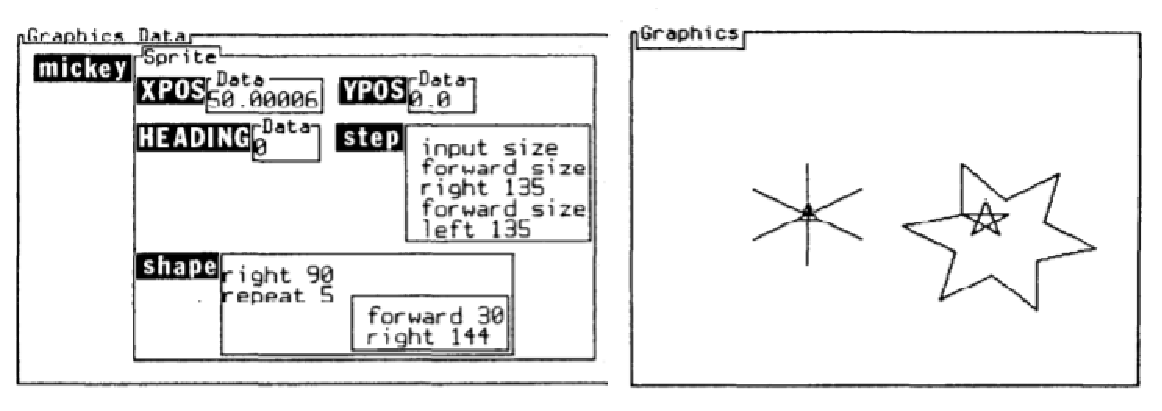
\includegraphics[scale=0.75]{images/CH2BOXER.pdf}
\caption{Graphical user interface for BOXER showing the graphics data (e.g., $x$-position, $y$-position, step instructions) and the resulting graphic for a sprite named mickey.}\label{CH2:BOXER}
\end{figure}

Alternatively, another implementation of computational physics takes the name VPython: the Python programming language with the Visual module.  Historically, the ultimate goal of developing VPython was to ``make it feasible for novice programmers in a physics course to do computer modeling with 3-dimensional visualizations \cite{Sherer2000}.''

Although VPython was ideal for novice programmers, it also catered to more advanced users.  Its basic algorithm is an Euler-Cromer style integration to calculate the contstantly updating position and momentum (or velocity) of an object within a while loop that depends on time.  For example, Fig.~\ref{CH2:MWP} shows the basic structure of a very simple but powerful MWP.  This Euler-Cromer algorithm can be used to analyze very simple situations (e.g., free-fall motion) as well as more complicated and realistic (e.g., the motion of satellites and rockets).

\begin{figure}\center
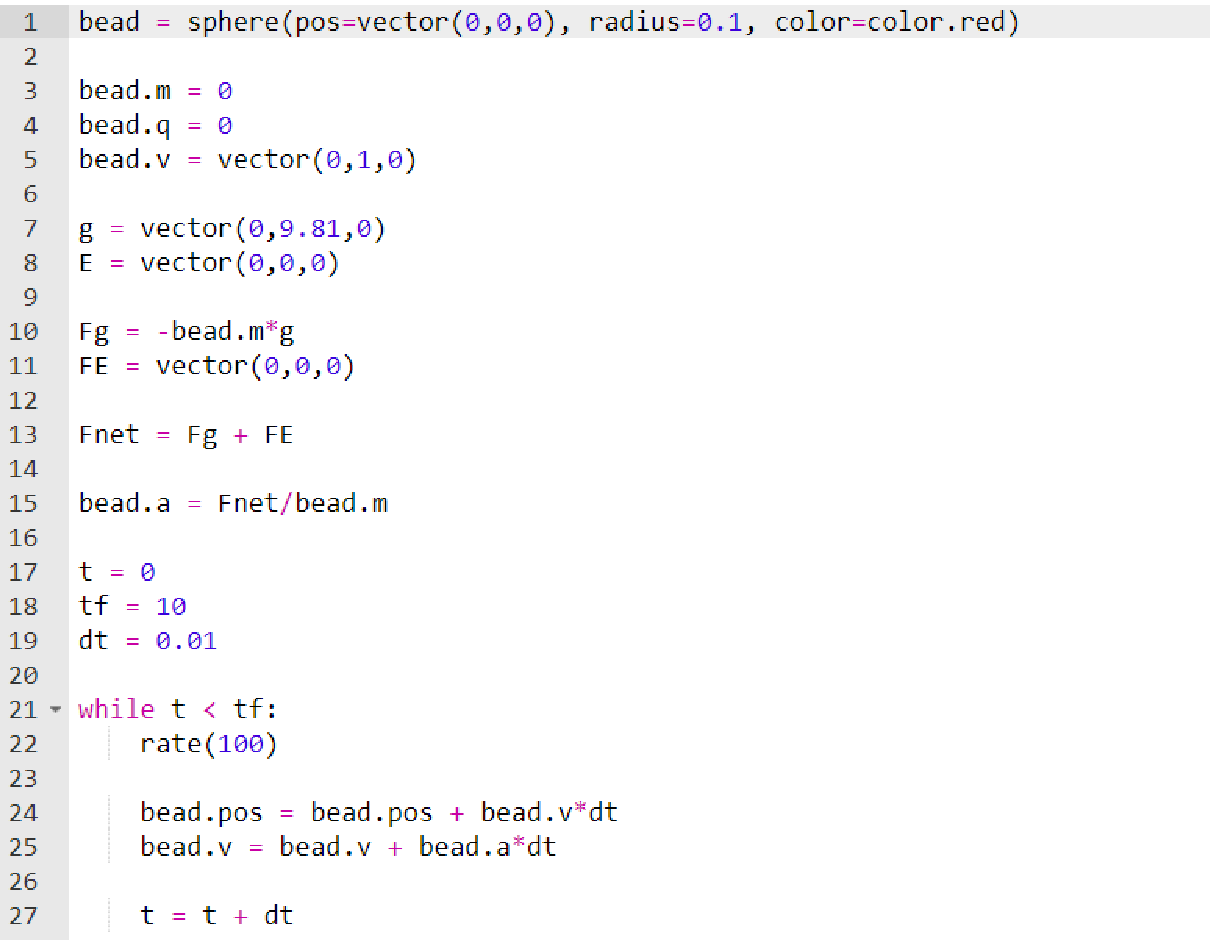
\includegraphics[scale=0.60]{images/CH2MWP.pdf}
\caption{A MWP illustrating that the basic control structure (while loop) and integration algorithm are pre-written so that students can focus on the computational force model that must be constructed in line 11.}\label{CH2:MWP}
\end{figure}

Along with the development of VPython, a software called Easy Java Simulations (EJS) was increasing in use \cite{Esquembre2005}.  These simulations were meant to give students a little more control behind the scenes, like VPython, while still limiting the generalizability like PhET simulations (described below).

For example, a simulation of a pendulum could be constructed in EJS by dragging a particular object (e.g, a pendulum bob) into the model and using their built-in editor to solve the associated differential equation (see Fig.~\ref{CH2:EJS}).  Only a small amount of modification is needed, reducing the load on novice programmers.  This reduction in load through scaffolded programs is very similar to the MWPs used in a lot of the research within PER \cite{Weatherford2011}.

\begin{figure}\center
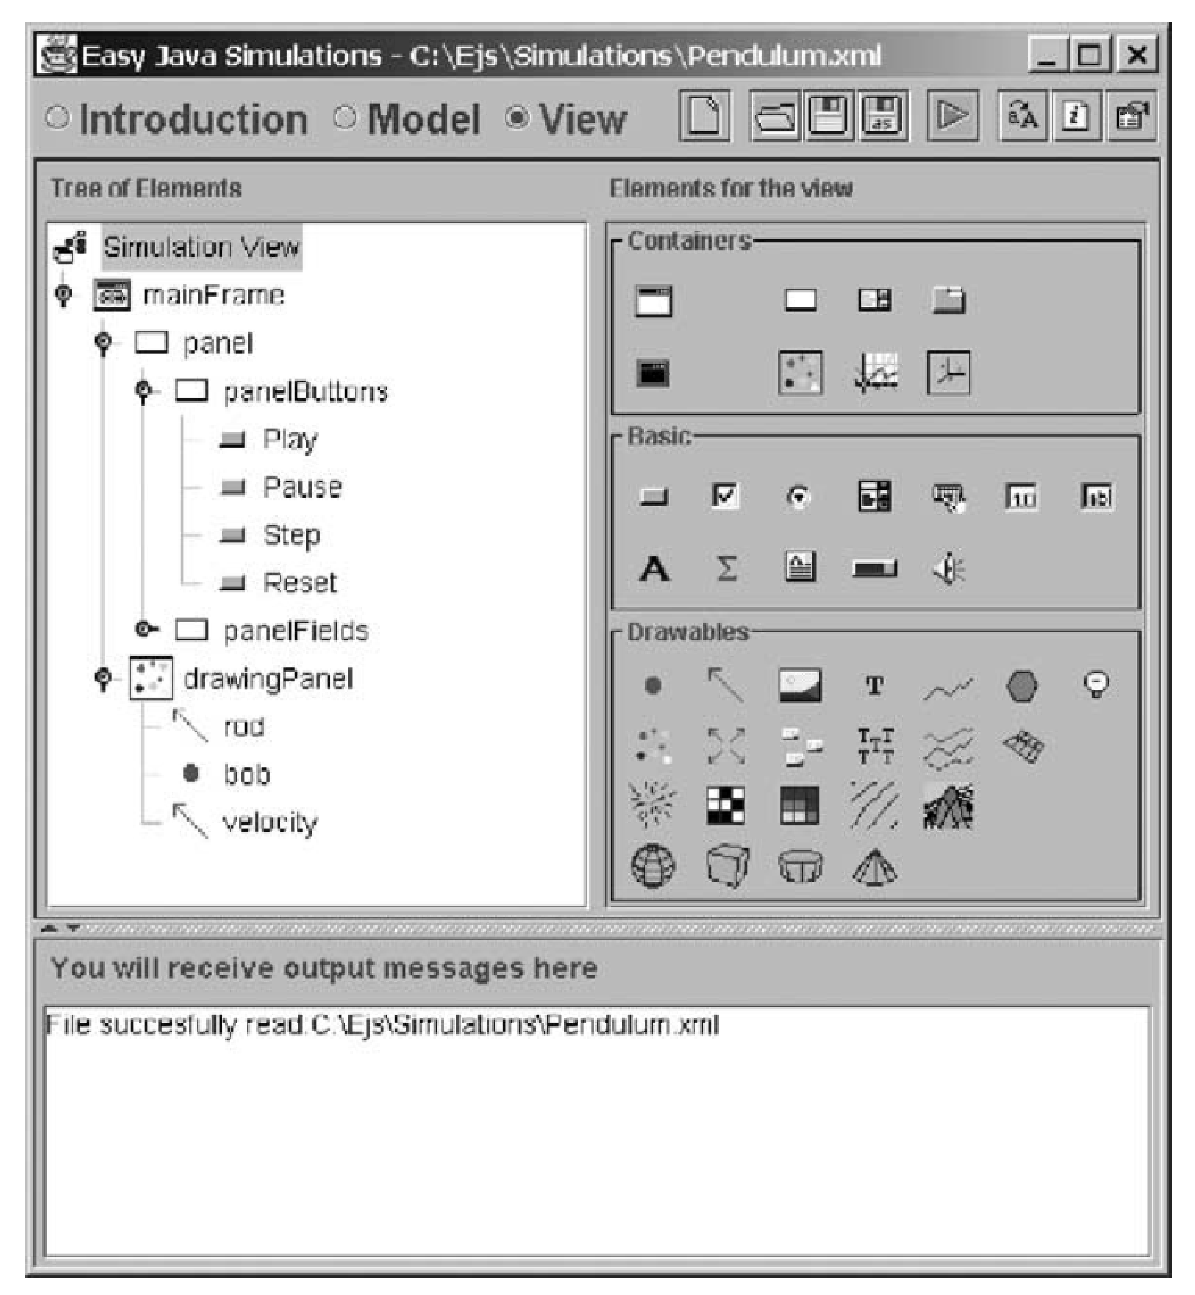
\includegraphics[scale=0.40]{images/CH2EJS.pdf}
\caption{Graphical user interface for an EJS illustrating the ``drag-and-drop'' nature of the software.  Elements (e.g., a pendulum bob) can be added or remove from the different panels (e.g., the drawing panel) in the simulation view.}\label{CH2:EJS}
\end{figure}

Another implementation of computation, frequently used today, are the Physics Education Technology (PhET) simulations \cite{Perkins2006}.  These simulations have realistic graphics that display buttons, sliders, and knobs that can be graphically tweaked to change parameters in a system.  This type of testing -- searching for the effect on a physical system with the variation in a parameter -- is meant to be more engaging and conducive to learning.

For example, the PhET simulation shown in Fig.~\ref{CH2:PhET} is meant to demonstrate the dependence of a pendulum's motion (e.g., its period or amplitude of oscillation) on the various parameters of the system (e.g., the length of the pendulum or the magnitude of friction).  Being able to hold one parameter constant while varying the other helps students to confidently identify its qualitative effect.

\begin{figure}\center
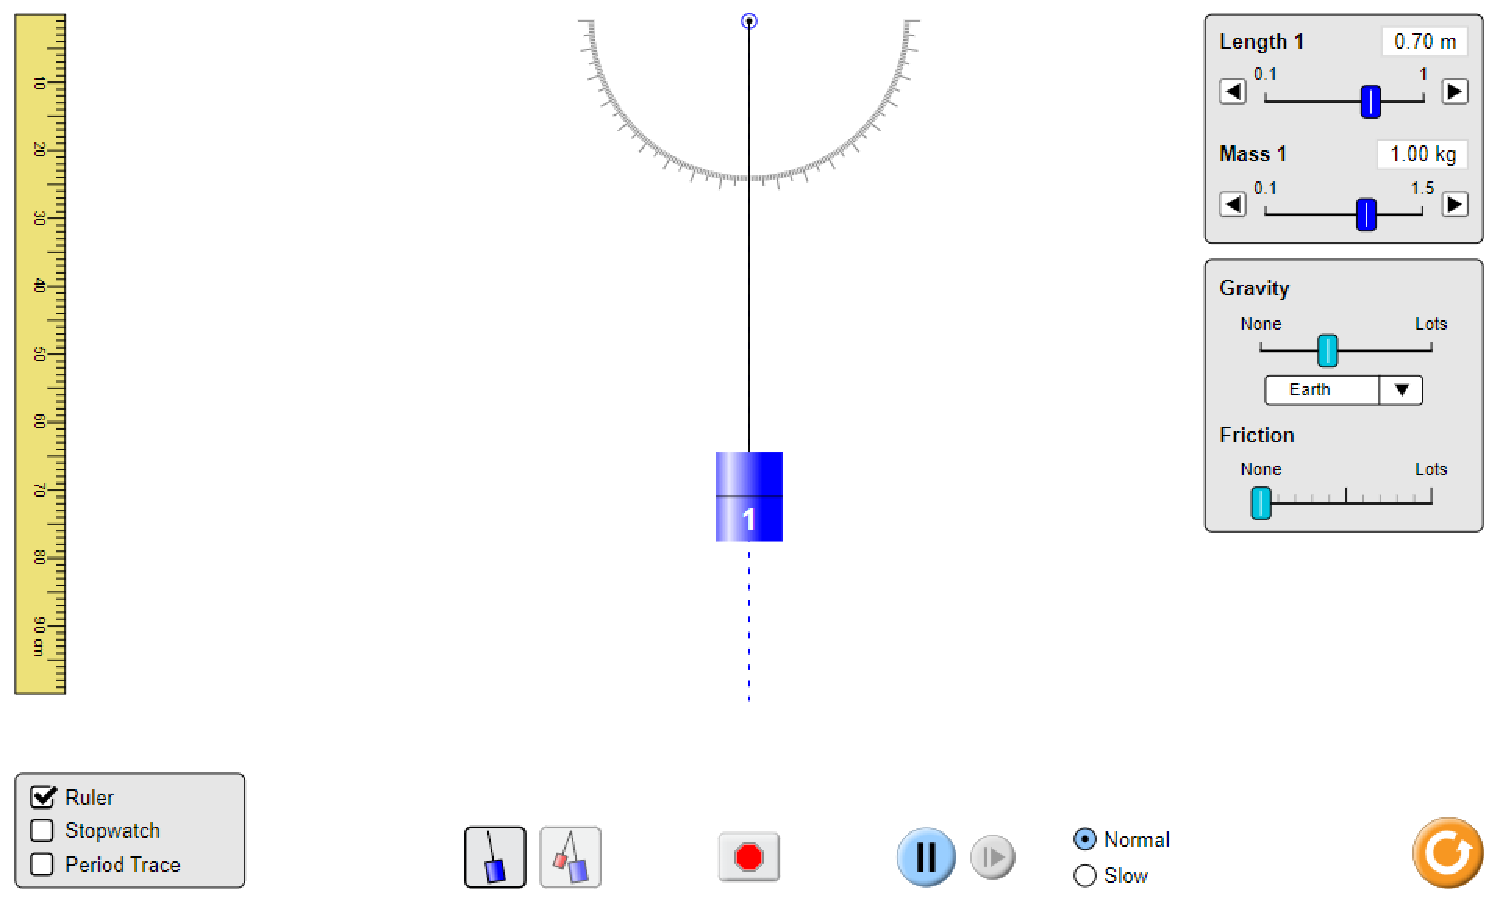
\includegraphics[scale=0.50]{images/CH2PhET.pdf}
\caption{A PhET simulation illustrating the dependence of pendulum motion on the length of the pendulum, the mass of the pendulum bob, the magnitude of the local acceleration due to the gravity, and any frictional forces.}\label{CH2:PhET}
\end{figure}

Finally, one of the more recent implementations of computation at the introductory level is called Glowscript \cite{Chabay2008}.  Glowscript is a variant of VPython which is designed, in part, to easily generate three-dimensional visualizations.  For example, the rather complicated Glowscript program shown in Fig.~\ref{CH2:Glowscript} uses an inverse-square electric field model with for and if loops to generate a visual representation of the electric vector field at any point in space surrounding a discrete charge distribution. 

\begin{figure}\center
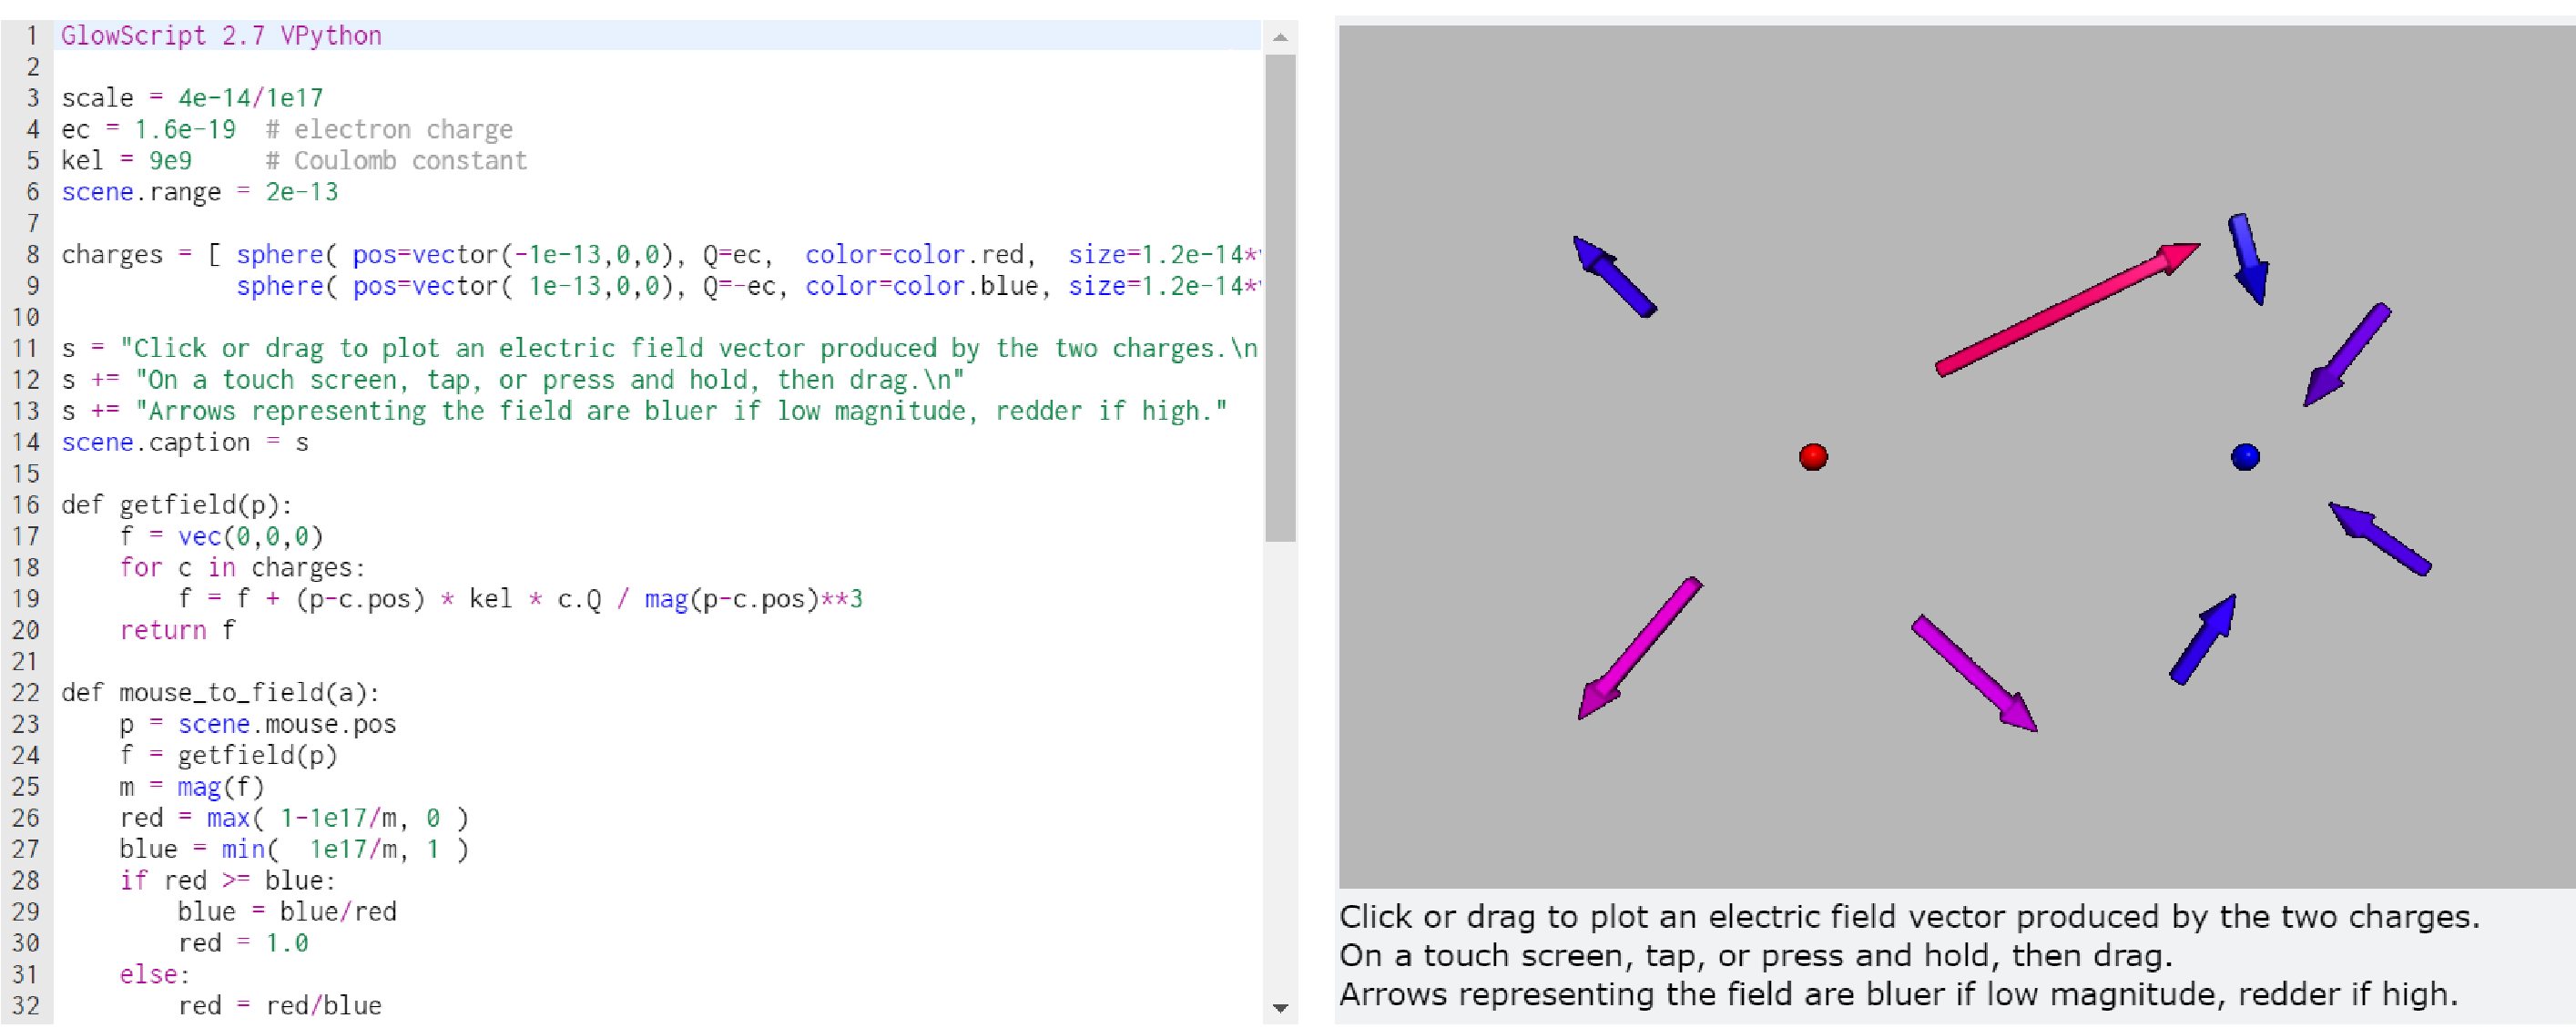
\includegraphics[scale=0.35]{images/CH2Glowscript.pdf}
\caption{Glowscript output demonstrating its ability to generate three-dimensional visualizations of objects, vectors, and graphs.  The ability to quickly and accurately generate three-dimensional vectors allows for more flexibility and a deeper understanding of, for example, electric (vector) fields.}\label{CH2:Glowscript}
\end{figure}

This more realistic and descriptive three-dimensional visualization leveraged by Glowscript and VPython is thought to encourage students to form a deeper understanding of the underlying physics concepts.  Although many different implementations of computation exist \cite{Papert1972,DiSessa1986,Perkins2006,Chabay2008}, research focusing on improving those implementations in PER is still lacking.  Some of the critical results, though, are described below.

\subsection{Results}

In the early 2000s, Chabay began to research the integration of computation into the introductory calculus-based physics course using VPython \cite{Chabay2008}.  This course included a computational curriculum following that presented by \textit{Matter and Interactions}.  Primarily, the courses studied by Chabay focused on the application of the integral equation governing the linear motion of objects (i.e., $d\vec{p}=\vec{F}_{\rm net}\,dt$ and $d\vec{r}=\vec{p}/m\,dt$).  These equations were applied iteratively through an Euler-Cromer style integration algorithm, and allowed a more thoroughly analysis of position-dependent forces (e.g., the Newtonian gravitational and spring forces).

Chabay found that one of the positive aspects of including computation at the introductory level was to stimulate creativity in students \cite{Chabay2008}.  This creativity in approaching problem solving is thought to lead students to the construction of more realistic computational models.  In other words, computation allows students to easily verify and/or modify a model, encouraging creativity and a ``guess and check'' approach to problem solving.

She also found that requiring students to program at the introductory physics level was a difficult barrier to overcome.  Given that there is so much content to be covered in so little time in most introductory physics courses, finding the room/time to discuss the basics of programming is difficult.  One of the ways in which this difficulty is overcome is by providing Minimally Working Programs (MWPs) to students.  The MWP for a particular problem usually runs without error from the start (pre-written code), and requires small (or at least localized) changes to the underlying computational models.  For example, see the MWP in Fig.~\ref{CH2:Caballero}.

Around that same time, Kohlmyer dug deeper into student performance \cite{Kohlmyer2005}.  He found that, among other things, computational modeling students struggled to recognize that computers could even be used to solve physics problems.  Furthermore, once they did decide to use a computer, they struggled with the concepts and components of creating a computational model.  These results were generated from two experiments: looking at how students approach novel problems with computation and looking at the differences in the fundamental principles used as compared to traditional (i.e., non-computation focused curriculum) students.

Interestingly, he found that students decided to take advantage of the Euler-Cromer style integration in discrete form even when they weren't using a computational model.  That is, students made use of the key conceptual tool that they were taught -- even if just on paper.

He also found that the complex procedure needed to model attractive position-dependent forces was a difficult challenge for students.  Reducing this and other difficulties can be achieved through increasing the frequency of computation throughout the course and requiring computational homework problems.  Kohlmyer made explicit the wide variety of unanswered questions that could be pursued in further research, hinting that the process of ``making assumptions'' and incorporating them into a computational model would be of particular interest.

In 2011, Weatherford began to look at integrating computation into the physics lab curriculum and the sense-making that students engage in \cite{Weatherford2011}.  His study was an in-depth qualitative analysis of group problem solving, focusing on three different contexts: a scattering problem, a spring-mass problem, and a spacecraft-Earth problem.  A coding scheme was developed to help categorize different portions of transcript, as shown in Fig.~\ref{CH2:Weatherford}.

\begin{figure}\center
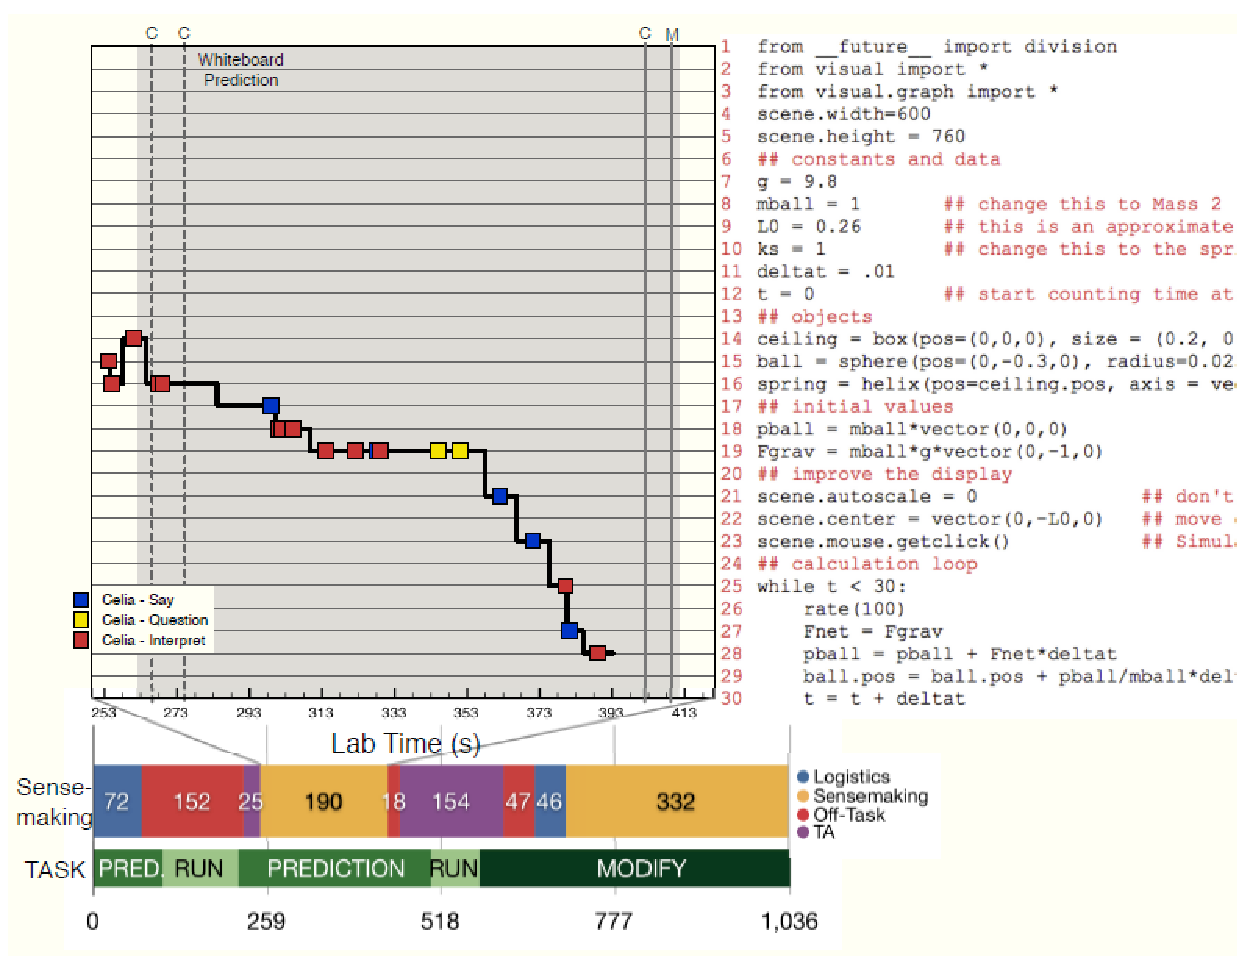
\includegraphics[scale=0.60]{images/CH2Weatherford.pdf}
\caption{A sample of the in-depth analysis Weatherford performed.  Each particular line of code that the group is focusing on is tracked in time and coded according to a scheme.}\label{CH2:Weatherford}
\end{figure}

He found, among other things, that computational physics students were able to reasonably interpret physical quantities according to their variable name.  For example, the mass of a satellite might be defined as \texttt{m.satellite = 1}, or the net force acting on object may be defined as \texttt{Fnet = vector(0,-m*g,0)}.  These pre-written variables are named so as to suggest to the students what physical quantity they represent.  However, the more complicated the definitions get (e.g., a function of multiple variables like \texttt{Fnet = -k * (ball.pos - origin.pos) / mag(L)}, the more students struggled at recognizing it.

Additionally, Weatherford was able to encourage students to begin to incorporate a computational model in a MWP by providing a minimum level of support.  That is, only omitting the fundamental physics calculations that students are meant to engage with (e.g., various computational force models) helps to keep students focused on the physics.  Other tasks that are not physical in nature have a tendency to derail the physics discussion and the problem solving process in general.  For example, ensuring that the end of a spring is connected to the end of a mass in a computational spring-mass analysis begins to overshadow the more fundamental task of incorporating/constructing a position-dependent Hookian spring force.  Alternatively, figuring out how to use the \texttt{mag()} function in Python can sidetrack the ultimate goal of constructing a position dependent gravitational force.

Weatherford clearly pointed out that the MWP activities in their study had much room for improvement, and that more research was needed on fostering student proficiency in computational physics.  The sequence of MWPs in his study didn't quite raise 
students' program comprehension and program interpretation skills to a certain profficiency, but he believes that more research will shed light on the subject.

In 2011, Caballero was able to identify a number of frequent student mistakes which were grouped into three different categories: initial condition mistakes, force calculation mistakes, and second law mistakes \cite{Caballero2011}.  An initial condition mistake might take the form of an incorrect initial velocity or momentum of the satellite.  A force calculation mistake might manifest in a constant spring force rather than a position dependent spring force.  A second law mistake might involve missing the division of the mass from the net force on an object so that the velocity is correctly updated according to the acceleration.  These frequent mistakes result in both unexpected and physically inaccurate visualizations.

Based on his analysis of the satellite-Earth problem, shown in Fig.~\ref{CH2:Caballero}, he concluded that the majority of students ($\sim\SI{60}{\percent}$) were able to correctly computational model novel physics problems and that the practice of debugging would serve students well.  Particularly, the act of troubleshooting syntax errors as well as the act of troubleshooting of \textit{physics} errors.

\begin{figure}\center
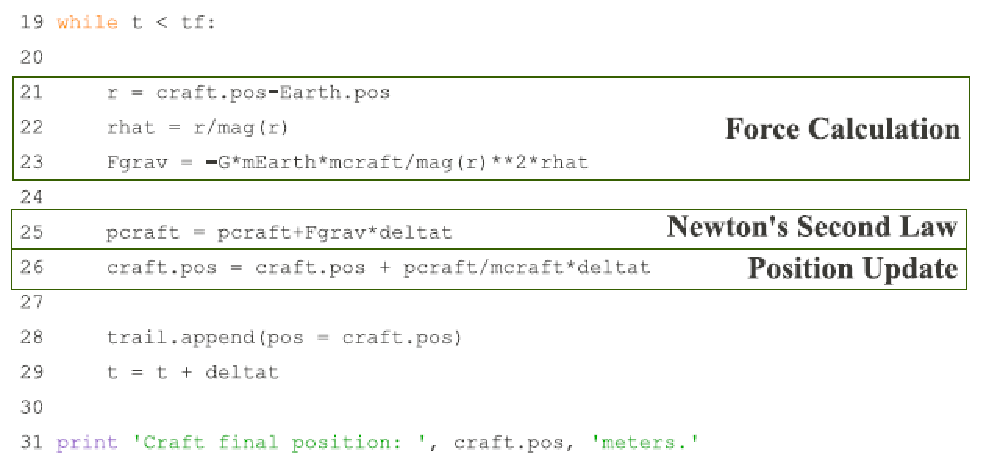
\includegraphics[scale=0.8]{images/CH2Caballero.pdf}
\caption{An expected solution to a computational satellite-Earth problem where the Newtonian gravitational force has been constructed from a separation vector and its magnitude.  The force calculation has been incorporated into the momentum through Newton's second law, and the momentum is incorporated into the position through a position update.}\label{CH2:Caballero}
\end{figure}

\subsection{Remaining questions}

Although many aspects of computation and computational thinking at the introductory level have been studied, there are still many unanswered questions within physics education.  Particularly, as to the types of practices students are engaging in that are indicative of computational thinking.  More research is needed to not only more clearly define the computational practices observed in introductory physics, but also to more clearly understand the habits of mind and types of thinking that students are engaging in.  \textbf{This thesis attempts to provide clear and precise definitions with examples of the various practices that students engage in within introductory physics.}

\section{Framework}

Recently, a framework for identifying the computational practices that are indicative of computational thinking has been proposed by Weintrop et. al.  This framework was developed using existing literature on computational thinking, interview with mathematicians and scientists, and most importantly, computational activities from general science and mathematics classrooms.

In order to develop their framework, a literature review was performed to generate an intial set of $10$ math and science practices.  These initial practices are repeatedly cited as being central to computational thinking.  For example, the broad and repeatedly cited practice of generating algorithmic solutions might require a student to engage with a differential equation algorithm.  These broad initial practices were used to guide the subsequent qualitative analysis.

Using the initial practices resulting from the literature review, two reviewers independently coded for the various ``facets'' of computational thinking that were required by the curricular materials.  They analyzed $32$ different computational activities from chemistry to programming, resulting in $208$ facets which were grouped into $45$ different practices.

Next, a review process incorporating feedback from multiple sources (e.g., teachers, content experts, and curriculum designers) was used to reduce the $45$ practices into $27$, which were further organized into $5$ different categories.  Further, external interviews were conducted with $16$ K-12 science and mathematics teachers, helping to reduce the $27$ practices into $22$ fitting $4$ different categories, shown in Tab.~\ref{CH2:Framework}.

\begin{table}[hb]\centering
\begin{tabular}{llll}\hline\hline
Data         & Modeling     & Solving     & Systems       \\\hline
Creating     & Conepts      & Preparing   & Investigating \\
Collecting   & Testing      & Programming & Understanding \\
Manipulating & Assessing    & Choosing    & Thinking      \\
             &              & Creating    & Communicating \\
             &              & Debugging   & Defining      \\\hline\hline
\end{tabular}
\caption{The framework developed by Weintrop et. al to describe the computational practices observed in science and mathematics classrooms.  Each category contains between five and seven individual practices, and each practice has between two and seven fundamental characteristics.}\label{CH2:Framework}
\end{table}

Finally, $15$ interviews with STEM professionals were conducted to rate their framework according to its appicability to authentic professional practices and to give direction for future improvement.  For example, interviews showed that the practice of testing and debugging was a crucial practice that was not adequately captured by the framework -- an improvement that should be made on future iterations of the framework.

The four different categories of practices are labeled as data, modeling and simulation, computational problem solving, and systems thinking practices.  The data practices focus mostly on the creation and visualization of data.  The modeling and simulation practices focus mostly on the design, construction, and assessment of a computational model.  The problem solving practices focus mostly on programming and debugging, while the systems thinking practices are a little more abstract and focus mostly on the structure of the program itself.

As a more concrete example, the computational practice of creating data (a data practice) has three fundamental characteristics: the creation of a set of data, an articulation of the underlying algorithm, and a use of the data to advance their understanding of a concept.  The more of the characteristics that we observe in a particular excerpt, the more confident we are that that excerpt can be classified as that practice.

Although each practice is defined like this, according to Weintrop et. al, the characteristics themselves are rather vague (similar to the operational defintions from the NGSS).  For example, the computational practice of assessing computational models requires the identification of a phenomenon, a computational model, and a comparison made between the two.  Although it is clear what a comparison would look like in any situation, the phenomena studied and the models used will depend greatly on the context (See Ch.~\ref{CH3:Context}).  For this reason, much more work must be done to clearly define computational thinking within introductory physics classrooms -- a central task to this thesis.

Ultimately, Weintrop found three main benefits to including computation: it builds on the reciprocal relationship between computationl thinking and STEM domains, it engages learners as well as instructors, and it introduces an authentic and modern element of doing science.  However, he is clear to indicate that more research is needed to better address the challenge of educating a technologically and scientifically savvy population.  This thesis attempts to improve that education process by providing clear and precise defintions with examples of the computational practices that are indicative of computational thinking.

\section{Task analysis}

A task analysis is a procedure that can be used to better understand the requirements of a particular task and the way an ``operator'' (or group of operators) might work to satisfy those requirements \cite{Kirwan2005}.  This type of task analysis is usually focused on the observable actions that an operator might engage in while working toward a particular goal (e.g., ), but there is also a strong cognitive link between the observed actions and the requirements of the task \cite{Crandall2006}.

Before begining a task analysis, data must first be collected.  Often, the method for collecting data is observation based (e.g., observing the actions of a group of operators as they carry out a task), although data can also be subject based (e.g., asking an expert what the ideal actions would be to carry out a task).  Either way, the task itself generally guides the collection of data.

Once the data has been collected, there are many different types of descriptions that can be attached to it and just as many techniques that can be used to generate them.  For example, one of the techniques frequently used is to \textit{chart and network} the data.  These descriptions can be written, but are most often presented visually through information flow charts or Murphy diagrams.  This thesis leverages a technique for generating an \textit{organized heirarchy} of description of the data: complex tasks are broken down into multiple smaller but more manageable tasks.

In order to give this research a solid foundation, early on, we conducted a task analysis of a complicated computational physics problem.  We wanted to look at what students were doing in a particular introductory physics classroom, and the task analysis was necessary to help guide our qualitative analysis.

Within an any particular classroom, there are a myriad of expected and unexpected tasks that students engage in while solving a particular problem.  For example, taking the time to name a variable with meaning, working to construct a multiple-variable function, or changing the color of an object within a program.  Given the almost limitless number of tasks that might draw students' (and our) attention, the task analysis was used to reduce the initial set of tasks that we focused our attention on.  This initial set of tasks was modified and expanded during subsequent qualitative analysis (see Sec.~\ref{CH2:Thematic}).

A task analysis consists of breaking a problem down into multiple smaller but manageable sub-tasks that can be tied together at the end.  This type of analysis is frequently used in the fields of mathematics and computer science \cite{Catrambone1998,Chandra1990,Fitzgerald2008,Ahmadzedah2005}.  The smaller but manageable sub-tasks are the ``unit of analysis'' that can then be searched for within data.  For example, an expert group might proceed in predicting the motion of an object by first constructing an Euler-Cromer style algorithm, constructing the various forces, and then construct the initial parameters of the system.  These steps can be done in any order, but are all necessary to the overarching task.

This type of process was used by Catrambone to show that breaking a problem down into smaller but manageable sub-tasks helps students to transfer knowledge to new and novel problems \cite{Catrambone1998}.  He and others believe that it is a heriarchical structure of tasks rather than a linear structure of tasks that students need to transfer knowledge to new and novel situations.  The flexibility of a heirarchical structure is thought to support a more varied approach to solving a problem.

\begin{table}[hb]\centering
\begin{tabular}{lr}\hline\hline
Step (Sub-Task) & Associated Code \\\hline
Construct separation vector & \begin{lstlisting}
sep = obj2.pos
\end{lstlisting}\\
between interacting objects & \begin{lstlisting}
         - obj1.pos
\end{lstlisting}\\\hline
Construct the unit vector & \begin{lstlisting}
usep = sep/mag(sep)
\end{lstlisting}\\\hline
Construct the net force & \begin{lstlisting}
Fnet = -G*m1*m2*usep
\end{lstlisting}\\
vector & \begin{lstlisting}
         /mag(sep)**2
\end{lstlisting}\\\hline
Integrate the net force over & \begin{lstlisting}
obj.p = obj.p + Fnet*dt
\end{lstlisting}\\
time into momentum & \\\hline\hline
\end{tabular}\caption{Some of the necessary steps that must be taken when constructing a Newtonian gravitational force in code.  Each step is associated with the construction/modification of a line of code.\label{CH3:TaskAnalysis}}
\end{table}

They performed three experiments, each focusing on how students transfer knowledge to new and novel problems.  The first experiment was a comparison between the meaningfulness of a label's name.  They found that the more meaningful the label was, the better prepared students were to solve new and novel problems.  The second was a deeper study of the connections between labels and sub-tasks.  They found, to a reasonable degree, that there was a fundamental connection between labels, sub-tasks, and how they were grouped.  The third was a talk-aloud study that looked at self-explanation while solving problems.  They found that aptly named labels could be used to cue students to group sub-tasks and explain their purpose through self-explanation.

The task analysis of the problem that this thesis focuses on was initially constructed by a single content expert.  After the first iteration it was presented to additional experts.  Through the discussions surrounding these iterations, it became clear that the construction of the position dependent Newtonian gravitational force in code is a multi-step procedure involving a number of different sub-tasks.  The task analysis was iteratively refined through this process until all experts agreed that the sub-tasks shown in Tab.~\ref{CH3:TaskAnalysis} were sufficiently described/defined to be useful in video analysis.
 
On top of this expert generated solution, there are many other (both expected and unexpected) student generated solutions that we observe in the data.  However, the expert generated solution is an ideal path to follow and so the instructors try to keep groups moving in this direction.  For example, a sufficient force model be constructed in terms of the polar and azimuthal angle of the satellite, although it requires a substantial amount of work to code.  Both the expert and student generated solutions are a good place to look for evidence of computational thinking and its accompanying practices.

\section{Thematic analysis}\label{CH2:Thematic}

Thematic analaysis is a poorly defined, but commonly used, type of qualitative analysis that is predominately used within psychology.  However, Braun makes the well-supported case that thematic analysis can effectively be used in many other fields (e.g., nursing or physics education) and clearly defines the sufficient steps that can be taken in order to complete a reasonably reliable and valid thematic analysis \cite{Braun2008,Fereda2006,Aronson1995,Vaismoradi2013,Joffe2004,Potter1997,Antaki2002}.

Within PER, thematic analysis is usually used for analyzing interview or work-aloud data of students solving problems.  For example, Irving found that there were many different themes that came from the various perceptions students have about what it means to ``be a physicist'' \cite{Irving2016}.  These themes were then broken down into $12$ sub-categories (e.g., high or low interest in research), highlighting the different perceptions students had about what it means to ``do physics.''  This type of analysis, as demonstrated by Irving, can be used to generate robust themes that can be used to inform instructional changes/improve instruction.

However, thematic analysis is just one of many qualitative techniques that can be used to analyze qualitative data.  The various qualitative methodologies can be broken into roughly two main types: those strongly tied to a theory/epistemology and those that are developed independent of a guiding theory/epistemology.  Thematic analysis, according to Braun, is of the second type.  So as to guard against the often cited critique of thematic analysis as being ill-defined \cite{Antaki2002}, Braun presents a 6-phase guide to conducting a reliable and valid thematic analysis.

According to Braun, a thematic analysis is a ``method for identifying, analyzing, and reporting patterns [themes] within data.''  This method consists of $6$ different phases, usually followed linearly, to finally produce a report (e.g., a thematic map) of the various themes and their relationships within a set of qualitative data.  However, before entering the first of the $6$ phases, there are a few fundamental decisions that must be made and explicitly stated.  Ideally, these decisions will be made in relation to the research question and the goal of the study.

First, it is crucial that researchers explicitly state the metric by which they plan to identify themes.  For example, a theme that shows up more frequently is not necessarily more important.  Additionally, a theme that shows up less frequently is not necessarily less important.  Rather, it is important to be consistent throughout anlysis.  This thesis mostly focuses on the more frequent themes, but consideration is also given to themes that are particularly illustrative yet infrequent.

Second, researchers must decide between a rich description of the entire data set or a more detailed account of a particular sub-set.  For example, within physics education, you might be interested in a rough description of the entire process that a group followed to successfuly solve a complicated problem.  Alternatively, you might want to focus in on a particular sub-task and its nuance.  Again, it is important to be consistent throughout your analysis.  This thesis focuses on a more detailed account of a particular sub-set of the themes (i.e., those involving computational thinking).

Third, researchers must decide between an inductive and a more theoretical approach to the generation of themes within their data.  An inductive approach often leads to themes that are not related to the original research questions, but rather have generated spontaneously and are more strongly ties to the data itself.  A theoretical approach, on the other hand, often leads to a set of themes that are less descriptive but are better suited to answer a particular research question.  Again, it is important to be consistent throughout your analysis.  This thesis follows a more theoretical approach, using the theoretical framework presented in Sec.~\ref{CH2:Framework} as a foundation for the generation of our themes.

Fourth, researchers must decide whether they will be looking for semantic or latent themes within their data.  Semantic themes are those that are clearly indicated within the data, whereas latent themes often go beyond what is actually being observed.  For example, within physics education, a group of students might be struggling with a particular problem.  The reason for this struggle might otherwise go unnotticed without looking beyond the immediate and recognizing that each student had a late and mentally taxing chemistry exam the previous night.  Usually a thematic analysis focuses on one level, and as always it is important to be consistent through your analysis.  This thesis primarily focuses on the semantic themes that are directly tied to the actions observed during the problem solving process.

Fifth, researchers must be choose between an essentialist and a constructionist thematic analysis.  An essentialist thematic analysis allows researchers to theorize student understanding and meaning in a straightforward way \cite{Potter1997,Widdicombe1995}.  A constructionist approach focuses more on the overarching sociocultural and structural environment that each student lives within.  It is important to be consistent throughout your analysis, and this thesis focuses on a more essentialist approach, paying special attention to the computational thinking and habits of mind that students are engaging in.

Once these decisions have been made, the qualitative analysis can proceed through the $6$ phases laid out by Braun.  The first phase focuses on (1) transcribing and farmiliarizing yourself with the data.  Reading through the transcripts multiple times helps to generate preliminary ideas that can be (2) coded for further investigation.  Next, each code must be (3) collated with the corresponding transcript so as to provide a context.  After the codes have been collated with the corresponding transcript, (4) themes begin to emerge in the third phase.  Reviewing any themes that emerge, particularly against the coded extracts and the transcript as a whole, leads to the next phase of (5) defining, validating, and naming any themes.  These themes can finally be presented in a (6) scholarly report with step-by-step transcript analysis and/or a thematic map.  A thematic map, like the one shown in Fig.~\ref{CH2:Map}, shows not only the components of a theme, but also the \textit{relationships} between those components.

\begin{figure}\center
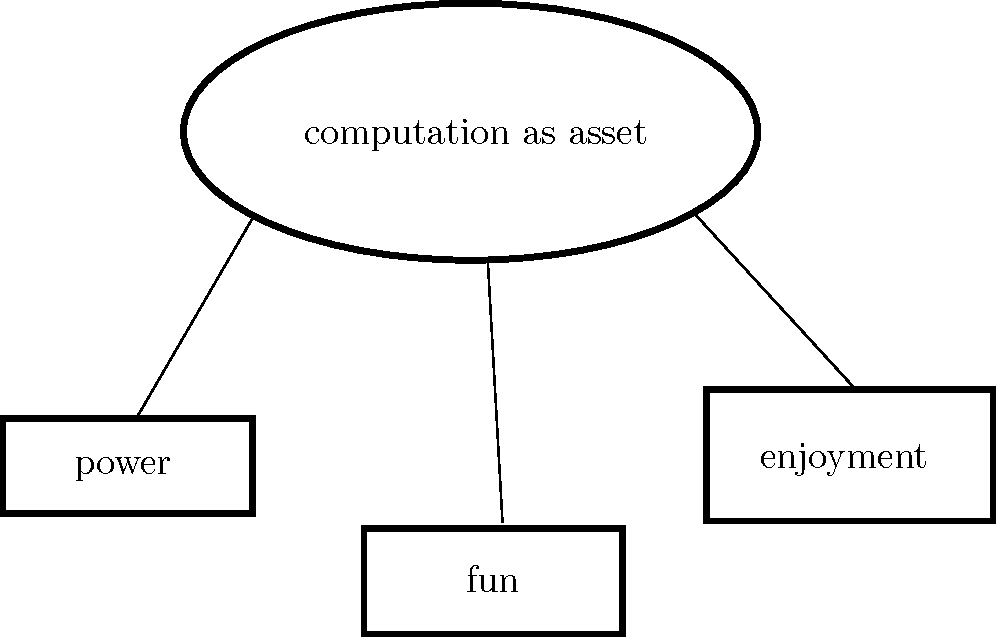
\includegraphics[scale=0.60]{images/CH2Map.pdf}
\caption{A final thematic map showing the components of a theme named ``computation as asset.''  The main components of this theme are ``power,'' ``fun'', and ``enjoyable.''}\label{CH2:Map}
\end{figure}

Braun is clear to point out that there are many pitfalls associate with thematic analysis, and that researchers must be cognizant of them through every phase of the process.  For example, one of the pitfalls she highlights is a possible mismatch between the data and the analytic claims that are being made.  In other words, it is important to always closely tie your claims with the actual data.  This closeness of the claims to the data can be ensured through frequent inter-rater reliability checks.

Given the flexibility of qualitative anlysis, it is important to be clear and explicit about the decisions being made throughout the entire process.  Braun has presented $15$ criteria for conducting a good qualitative thematic analysis.  These criteria focus on things like checking that each data item has been given equal attention, and checking that themes are internally coherent, consistent, and distinctive.  These critera help to safeguard against the many pitfalls of thematic analysis.

As we have shown, thematic analysis is a powerful and flexible qualitative methodology.  Accordingly, this thesis leverages thematic analysis to guide our study of group problem solving in introductory computational physics with the hopes of highlighting the various practices students engage in that are indicative of computational thinking.  A detailed account of this process is described in Sec.~\ref{CH5:Observations}.

%
%
%
%
%
%
%
%
%	CONTEXT (P3)
%
%
%
%
%
%
%
%

\chapter{Context}\label{CH3:Context}

It is important to understand the course from which we have collected our data to better understand the results of our study.  That course -- called Projects and Practices in Physics (${\rm P}^{3}$) -- is based on a social constructivist theory of learning and a flipped/problem-based pedagogy \cite{Irving2017}.  In other words, students familiarize themselves with relevant material before coming to class, where they will work in small groups to actively and socially construct knowledge while solving complex analytical and computational physics and engineering problems.  The course has intentionally been designed to encourage computational thinking wherever possible.  Specifically, computational thinking has been incorporated into the notes, pre- and post-class homework, in-class feedback and assessments, and a selection of the in-class problems.

\section{Course design}

Each week in ${\rm P}^{3}$, students are expected to do a number of things. They must complete the pre-class homework which is based on information that they should gather from the pre-class notes.  They must then work in small groups (usually between three and four members) on two related analytical problems or a mixture of one related analytical and one related computational.  These problems are delivered during the two two-hour weekly meetings (See Fig.~\ref{CH3:Schedule}).  For the computational problem, that means reading and interpreting pre-written code (i.e., a minimally working program) while they design, assess, and construct a computational force model.  The small group is facilitated by either a course instructor, graduate teaching assistant, or undergraduate learning assistant who will ask relevant and pertinent follow-up questions.  There are also post-class homework questions based on information gathered from the pre-class notes and the in-class problems that are due at the end of the week.  This all occurs while students simultaneously prepare for the following week.

\section{VPython}

Given that the vast majority of students enter ${\rm P}^{3}$ with little to no prior programming experience, we need to ensure that they are prepared to handle computational problems early in the semester.  One way that we can ensure this is by requiring students to engage with the fundamental programming ideas (e.g., iteration through a while loop control structure or pre-defined mathematical functions) before coming to class through pre-class homework and notes.  These notes and homework questions highlight the fundamental physical and programming ideas specific to VPython and the computational problems that will be delivered in class.

For example, consider the portion of the course notes shown in Fig.~\ref{CH3:VPythonNotes}.  These notes are made available to the students at the beginning of the semester and are meant to provide students with a basic understanding of the utility of VPython along with a list of common errors that novice programmers must frequently deal with.  These notes provide not only a description of the error, but also a procedure for removing it while students are troubleshooting and debugging in-class code.  Troubleshooting and debugging are two of the problem solving practices indicative of computational thinking that we focused our analysis on.

\begin{figure}[ht]\centering
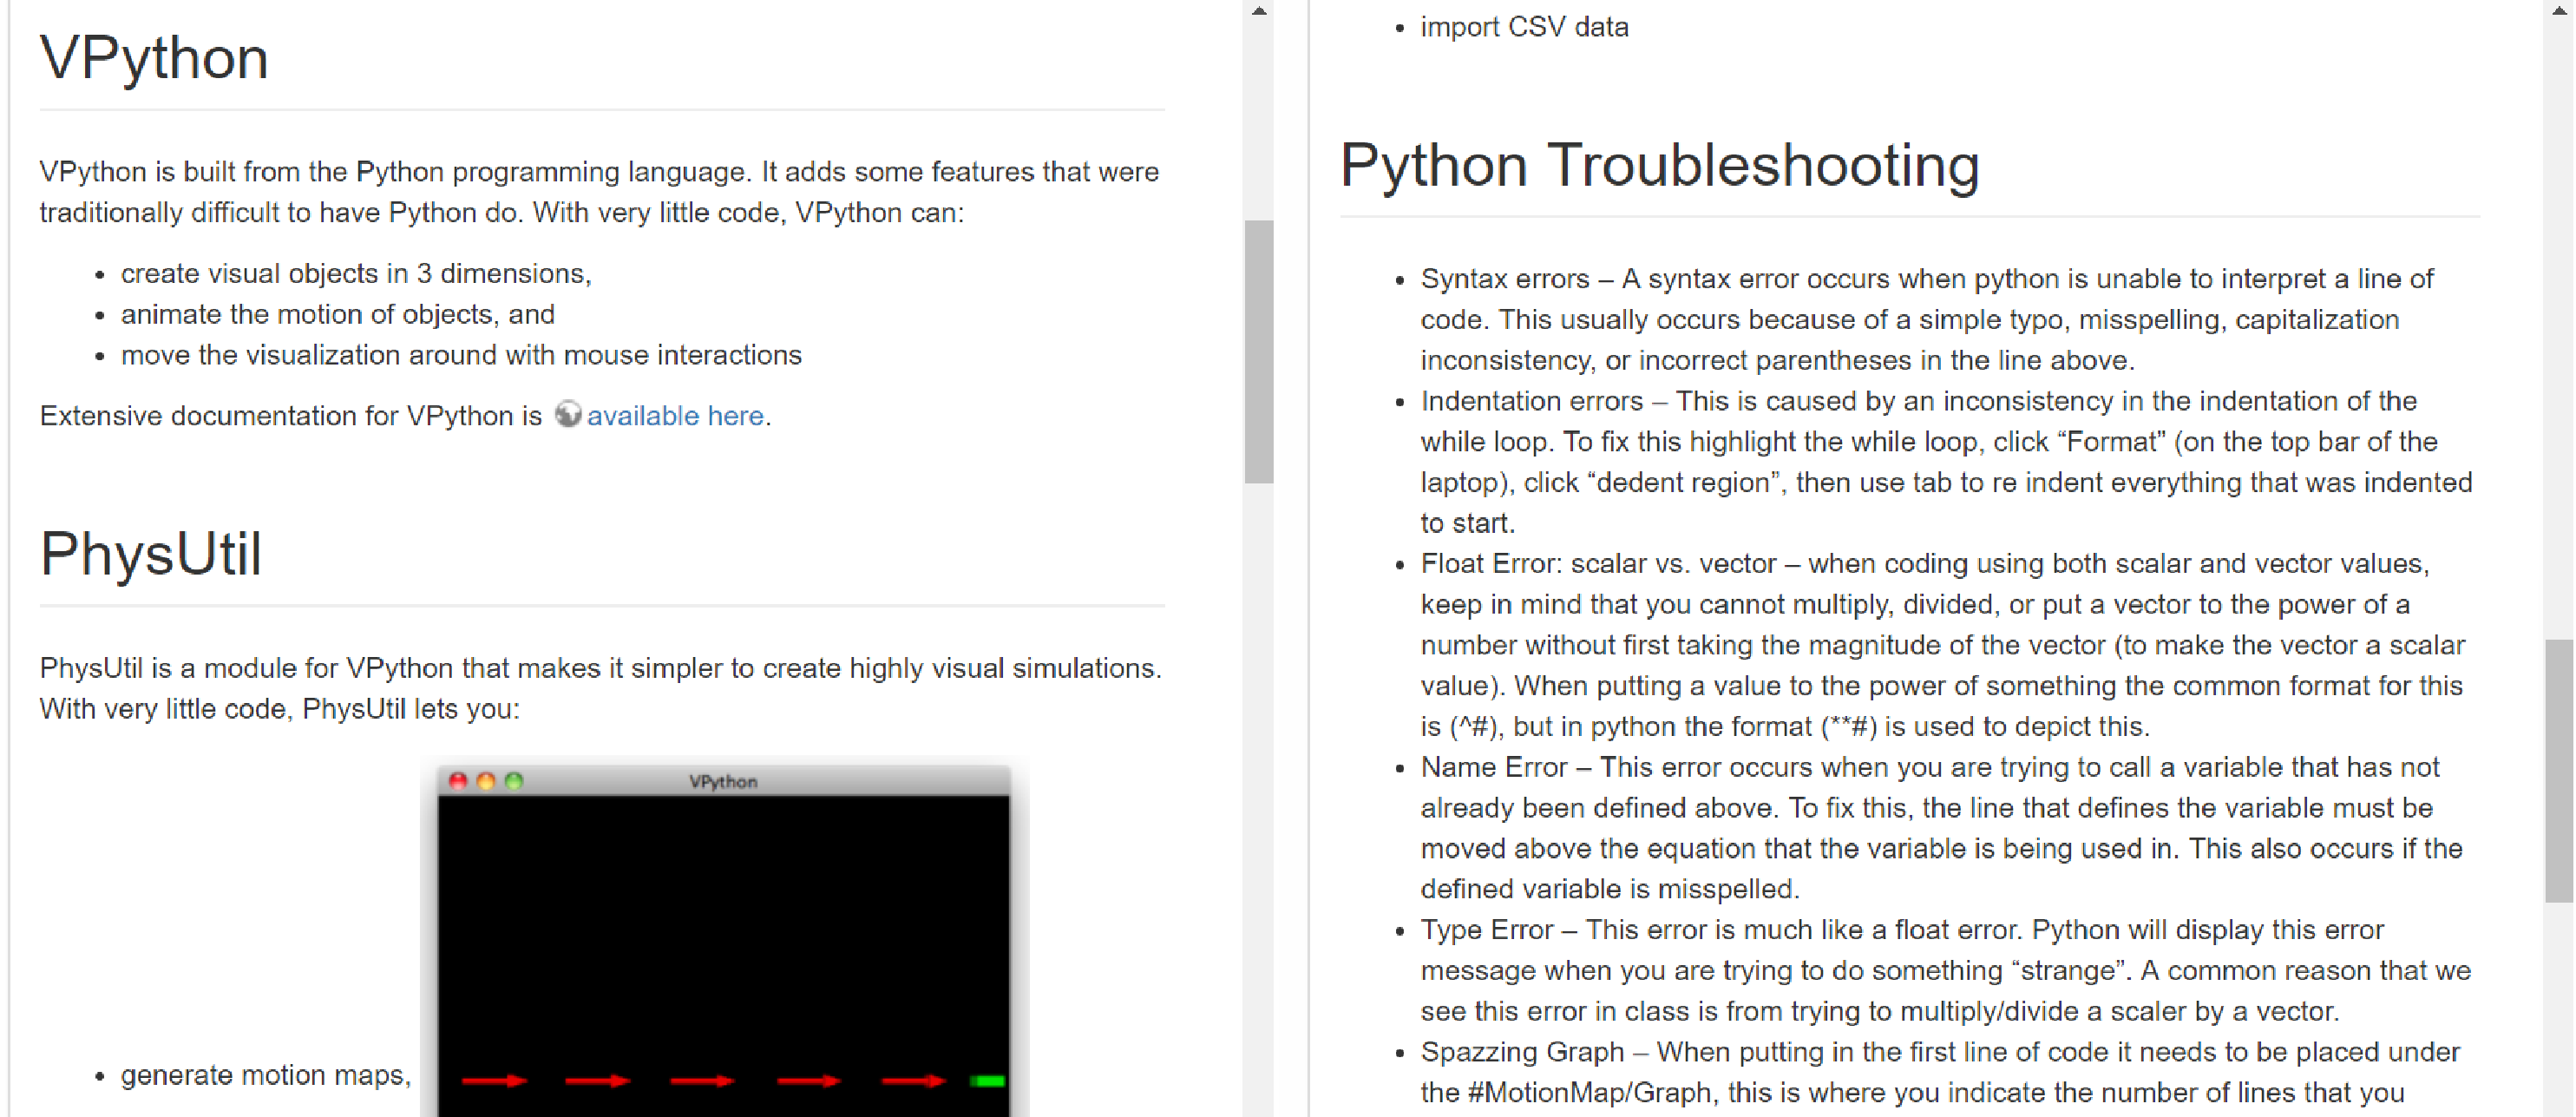
\includegraphics[scale=1]{images/CH3VPythonNotes.pdf}
\caption{Portion of on-line notes that is made available to the students during the first week of the course.  These notes introduce the fundamenatal programming ideas and a list of common errors with tips and tricks.}\label{CH3:VPythonNotes}
\end{figure} 

\section{Pre-class work}

There are other weekly notes, made available to the students at the beginning of every week, focusing more on the fundamental physical ideas that will be used during class.  For example, during the third week the notes focus on uniform circular motion (most heavily used during the week's analytical problem) and the Newtonian gravitational force (most heavily used during the week's computational problem).

Aside from notes, material is also delivered to the students through weekly pre-class homework questions.  Consider the pre-class homework questions shown in Fig.~\ref{CH3:PreClassQuestion} that are made available at the beginning of the third week of the course.  This question is meant to demonstrate that there are multiple correct ways that a unit vector can be constructed in code.  Given the nature of the corresponding week's computational problem (see Sec.~\ref{CH3:SatelliteProblem}), we expect students to be able to draw on and take advantage of this knowledge when faced with a related albeit more complicated problem.  That is, we expect students to be choosing between competing solutions.  Choosing between competing solutions is a problem solving practice indicative of computational thinking that we focused our analysis on.

\begin{figure}[ht]\centering
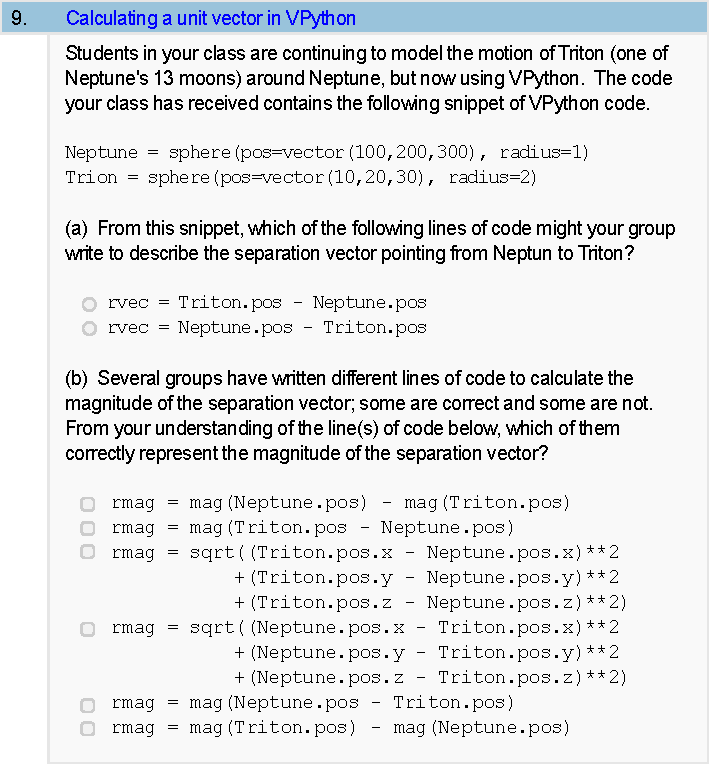
\includegraphics[scale=0.75]{images/CH3PreClassQuestion.pdf}
\caption{Pre-class homework question focusing on the different ways that the magnitude of a vector can be constructed in VPython code: explicitly coding the square root of the sum of the squares of the components and using the pre-defined Python ``magnitude'' function.}\label{CH3:PreClassQuestion}
\end{figure} 

Targeted pre-class homework questions were also developed to help students overcome challenges based on the task analysis.  For example, the pre-class homework questions shown in Fig.~\ref{CH3:PreClassQuestion} were developed to facilitate student understanding of the unit vector of a separation vector between two objects prior to working on the related computational problem.  Given that students must grapple with using a separation vector to construct a unit vector in code during the week, these questions help to place them in the Zone of Proximal Development (ZPD) \cite{Vygotsky1980}.  Constructing computational models is (unsurprisingly) a computational modeling practice indicative of computational thinking that permeates our data.

\section{In-class work}

There are a number of in-class computational problems spread out throughout the semester (see Fig.~\ref{CH3:Schedule}).  The first few computational problems focus on different force models (i.e., no force, a constant force, a non-constant force) and the resulting linear motion of objects.  The last few computational problems focus on extended objects and their rotation.  While solving these problems, groups are expected to engage in a number of computational practices that the problems have been designed around: \begin{enumerate}
\item[P1.] developing and using models,
\item[P2.] planning and carrying out investigations,
\item[P3.] analyzing and interpreting data,
\item[P4.] using mathematics and computational thinking,
\item[P6.] constructing explanations,
\item[P7.] engaging in argument from evidence.
\item[P8.] and obtaining, evaluating, and communicating information.
\end{enumerate}

%\begin{landscape}
%\thispagestyle{empty}
\begin{figure}[ht]\centering
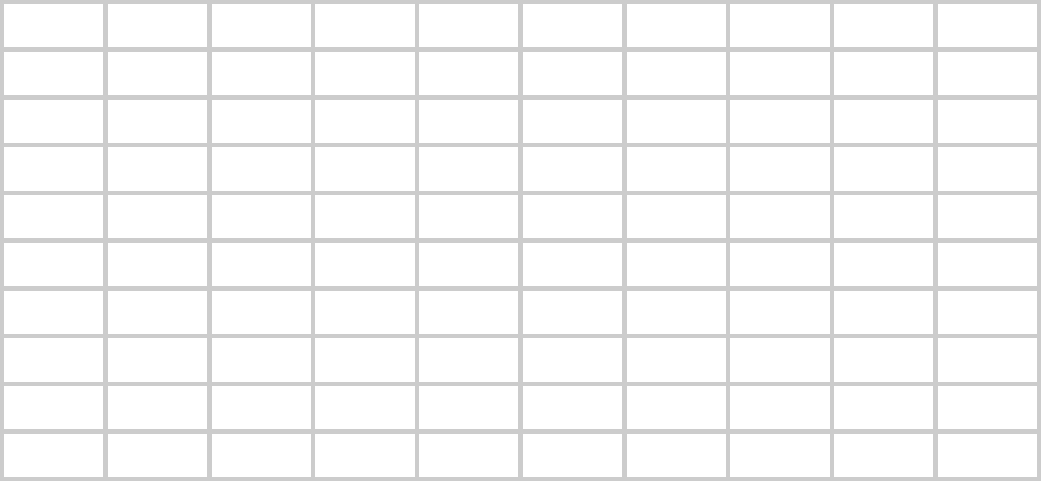
\includegraphics[scale=0.60]{images/CH3Schedule.pdf}
\caption{A schedule for the semester focusing on topics covered, homework/reading deadlines, and in-class problems.  \textbf{Should this figure be on a landscape page?}}\label{CH3:Schedule}
\end{figure}
%\end{landscape}

One of the scientific practices used heavily on both analytic and computation days is that of (P1) developing and using models.  Whether those models be mathematical or computational, we expect students to not only work together in groups to develop the model, but also to utilize that model in further investigations.  This type of scientific practice (P1) and its associated learning goals \cite{Irving2017} were further used to generate the in-class project that this thesis focuses on.

\subsection{Analytic problem}

In the third week of the course, students are asked to analyze the motion of a satellite orbiting Earth both analytically and computationally.  For the analytic day, the groups were asked to solve for the magnitude of the velocity and radius needed by a satellite to be held in a geostationary orbit.  This involves identifying two relevant equations in two unknowns and combining them to solve for the desired radius and magnitude of velocity.  The information gathered during this problem can be used in the following computational problem, and the group facilitators are often observed referencing this information.

\subsection{Computational problem}

This thesis focuses on the third and most complicated computational problem delivered to the students, shown in both Figs.~\ref{CH3:Schedule} and \ref{CH3:SatelliteProblem}. Given its complexity, we developed a framework to help guide and ground our analysis.  This framework was constructed with the help of a task analysis (see Sec.~\ref{CH2:Background}) of the problem.  Ultimately, students must design, construct, and asses a computational model for the Newtonian gravitational force acting on a satellite in geostationary and other more general orbits.

\begin{figure}[ht]\centering
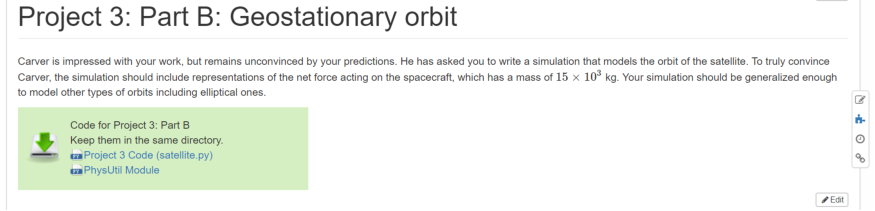
\includegraphics[scale=1]{images/CH3SatelliteProblem.pdf}
\caption{The Newtonian gravitational force problem statement delivered to the students in the third week of class.}\label{CH3:SatelliteProblem}
\end{figure}

Once the correct force has been correctly coded, the group must also grapple with adding in a visualization of a vector representing the force that they have just added.  This type of motion diagram is meant to show that the gravitational force vector resulting in the orbit always points radially inward (toward the Earth).  This task requires students to program as well as allows them to more easily check their conceptual understanding.  Using computational models to understand a concept is a computational modeling and simulation practice that is indicative of computation thinking.

Additionally, in order to check that their model can produce a geostationary orbit, groups are asked to generate a graph showing the magnitude of the separation between the satellite and the center of the Earth vs. time.  This allows them to check for a constant distance which implied a circular orbit.  This task is meant, among other things, to encourage students to visualize data, another computational practice indicative of computational thinking.

\subsubsection{Minimally working programs}

While beginning the problem, the group will observe a Minimally Working Program (MWP) similar to those seen in the two previous computational problems.  This MWP has all of the structure of the code correct (the while/calculation loop and the Euler-Cromer integration) but is missing the computational force acting on the satellite (along with some inaccurate numerical values).  The initial MWP code with its initial visualization are shown in Fig.~\ref{CH3:InitialCodeVisual}.

\begin{figure}[ht]\centering
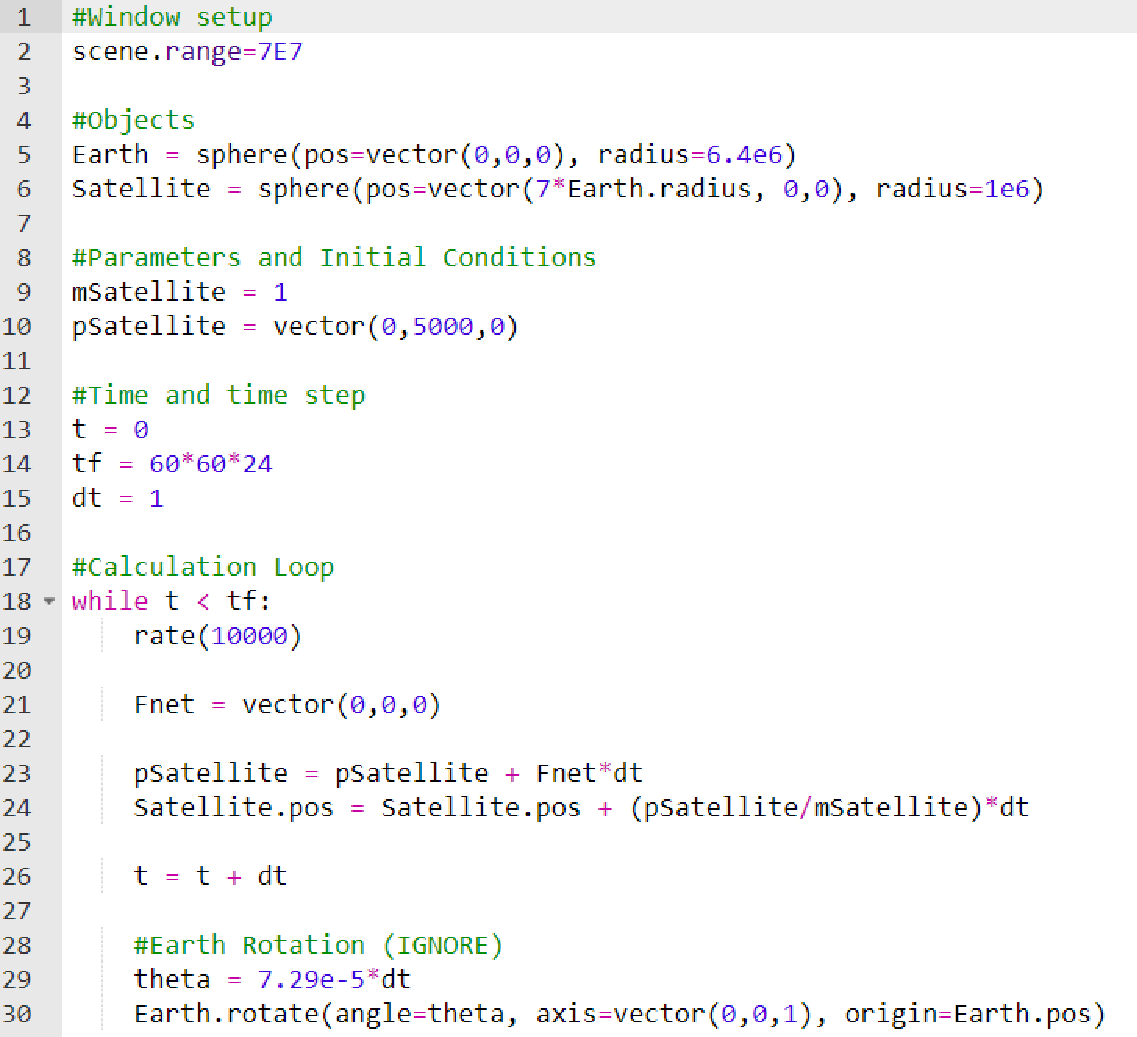
\includegraphics[scale=0.40]{images/CH3InitialCode.pdf}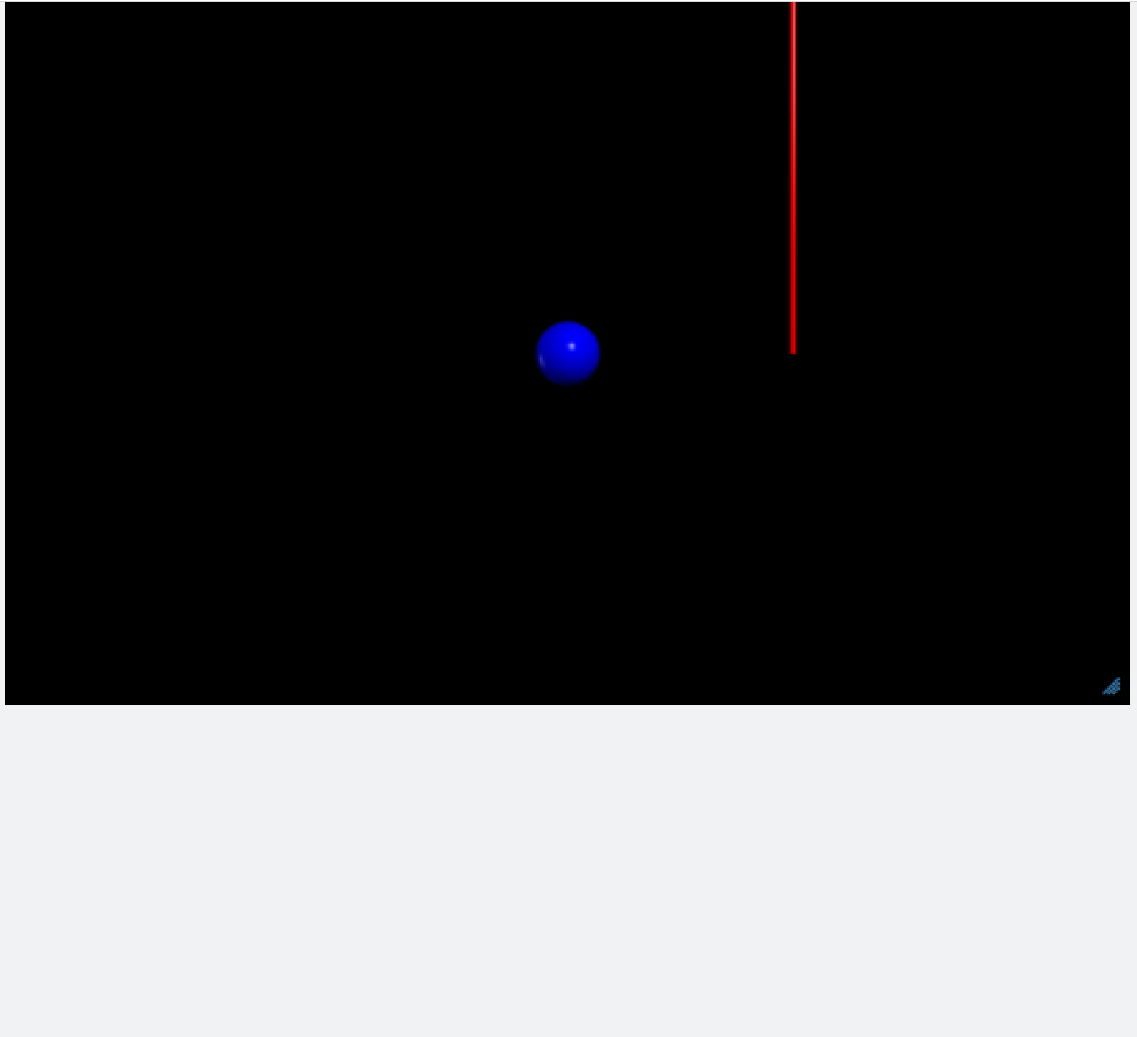
\includegraphics[scale=0.40]{images/CH3InitialVisual.pdf}
\caption{The initial code and visualization of the MWP that is given to the students in the third week of the course.}\label{CH3:InitialCodeVisual}
\end{figure}

Thus, the main task of the group is to construct a physically correct force model in code.  Secondarily, they must modify numerical values to reflect the phenomenon being modeled.  Ideally, this force model will be of a Newtonian gravitational form (i.e., $F_{G}\sim1/r^{2}$) with a direction coded in terms of a separation vector (i.e., $\hat{F}_{G}\sim\vec{r}/r$).  However, there are many other ways to go about this, and we do frequently observe groups working with other models (e.g., a centripetal force).

\subsubsection{Tutor questions}

There are a number of pre-written tutor questions as well as many on-the-fly questions generated by the tutors while in class.  These questions are meant to check the students for conceptual understanding as well as to direct students toward the correct solution.  For example, the tutor questions shown in Fig.~\ref{CH3:TutorQuestion} are meant to ensure that the model the group has constructed is actually general enough to generate all types of elliptical orbits given various initial conditions.

\begin{figure}[ht]\centering
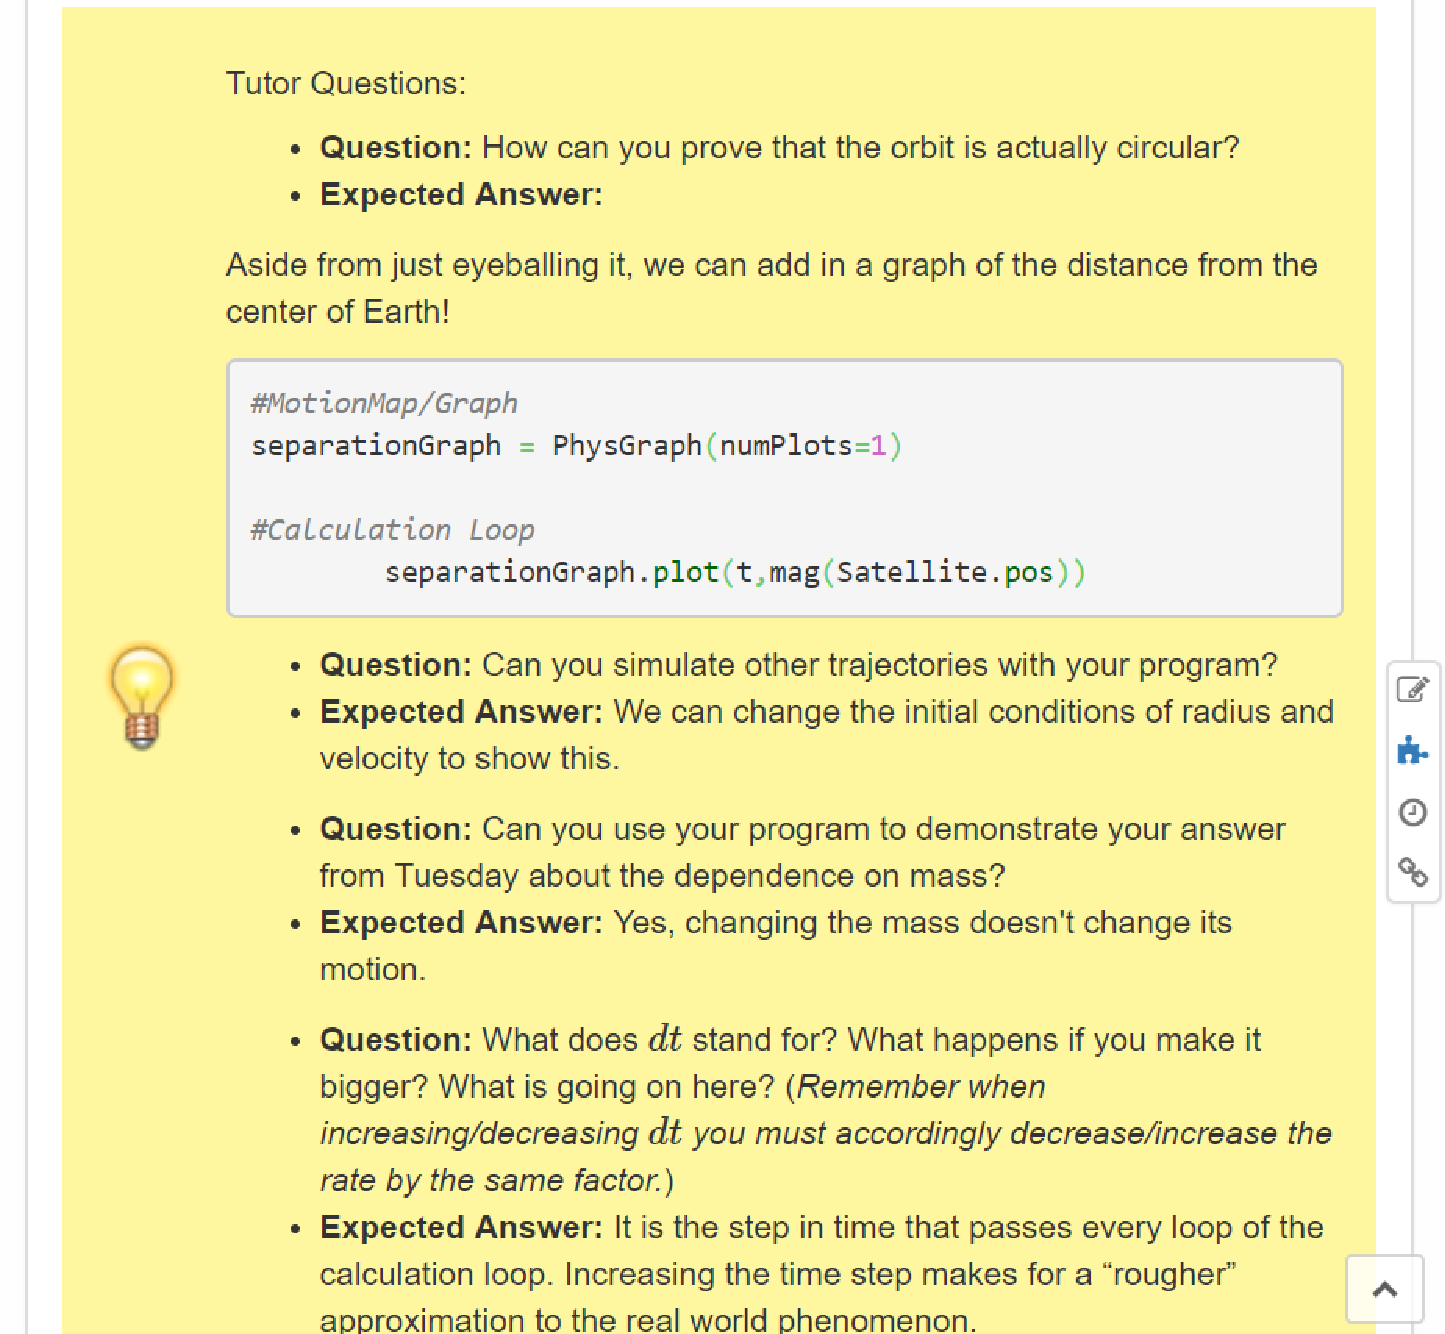
\includegraphics[scale=0.5]{images/CH3TutorQuestion.pdf}
\caption{A seclection of tutor questions that focus on the computational model each group has constructed.}\label{CH3:TutorQuestion}
\end{figure}

On the other hand, a tutor interaction like the one shown below that happens on-the-fly might encourage students to use a more general force rather than a more restricted one:  \begin{description}\TA  you guys wanna talk about what your trategy is at hte moment
\SB  i dont think we know	
\SA we just, we need to figure out how to get the velocity of the spacecraft correct as well as the force net correct and then it should be fine				
\TA yeah, my request, can i point in your program thats what you have for F net now [constant components] my request is to use a completely different strategy where that formula [points to Gmm/r2 on the board] is in for Fnet
\SC yeah we tried to make that yeah		
\SA can we just put the number in?				
\TA umm in principle you could, but id really rather you not have you do it i would like the program to be able to respond if the satellite is father away the force would be less, if the satellite is closer the force would be more so i would like it to be a dynamic program and not one that always have a fixed force\end{description}  In this on-the-fly interaction, the question of weather or not their computational model will be able to handle all types of orbits is enough to indicate that the group needs to switch their model up.  In this way, the tutor is able to make sure the groups stay on the desired path without directly telling them exactly what to do.

\subsection{Feedback/Assessment}

The groups are assessed on many levels in ${\rm P}^{3}$.  One of the most important forms of assessment is given weekly, in the form of written feedback and a numerical score.  The written feedback is based on the observed in-class performance and is designed to point out deficiencies and suggests ways to improve.  The numerical scoring is based on performance in three categories: group understanding, group focus, and individual understanding.

Often the written feedback pertains to group activity with the computer.  For example, the portion of written feedback shown in Fig.~\ref{CH3:WrittenFeedback} is encouraging a student to allow other group members to do some of the typing.   This could be requested for any number of reasons -- most likely, though, because the students with less prior programming experience are not being given a chance to participate.

\begin{figure}[ht]\centering
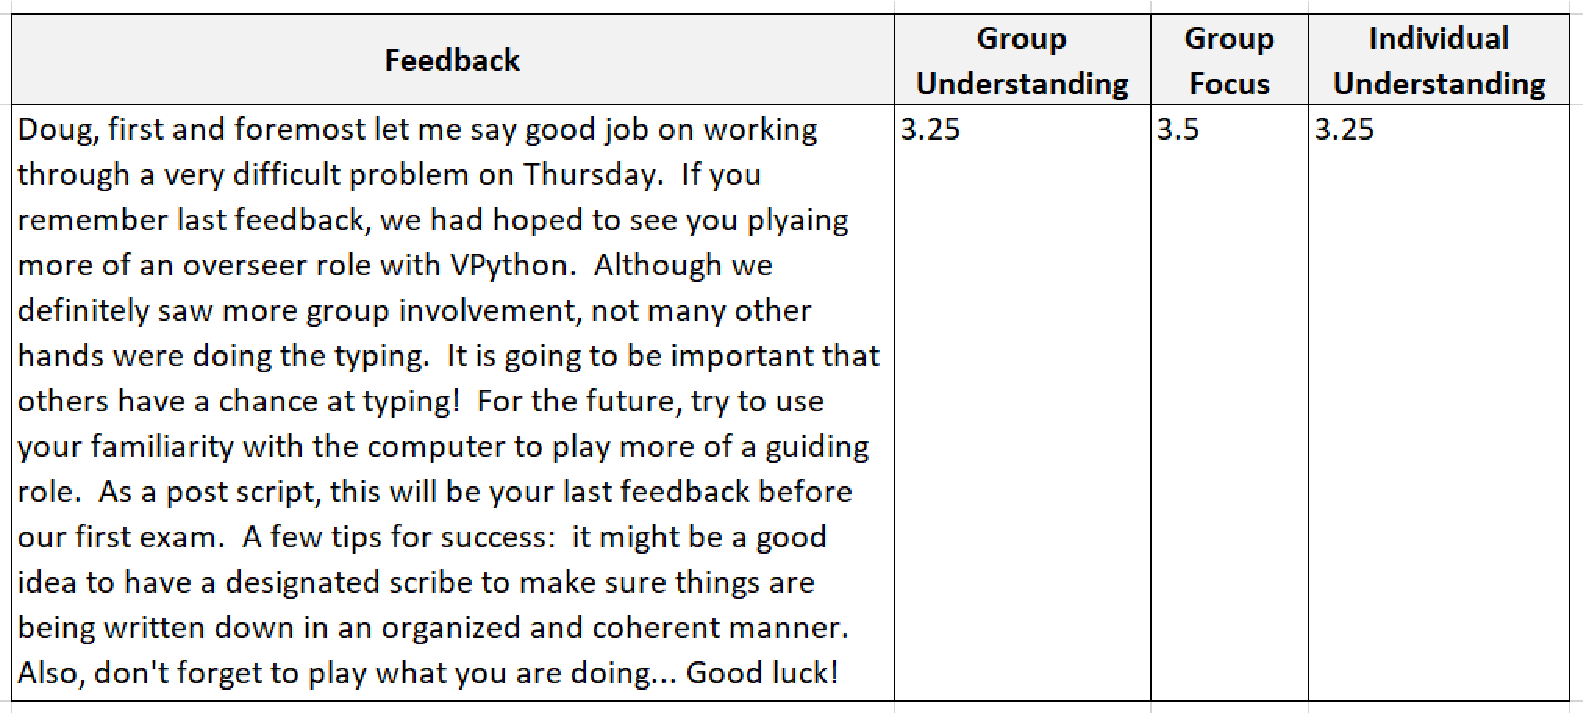
\includegraphics[scale=1.25]{images/CH3WrittenFeedback.pdf}
\caption{A snippet of written feedback given to a student after the third week.}\label{CH3:WrittenFeedback}
\end{figure}

In this way, instructors can encourage their groups to share the programming load.  While doing the typing, it is very difficult to follow along without knowing exactly what is going on.  This helps to engage all of the students with the material.

\section{Post-class work}

There are a number of post-class homework questions that are meant to reinforce the physics and computational concepts seen in class.  During the third week of the course, these questions focus mostly on the Newtonian gravitational force.  However, the post-class homework question shown in Fig.~\ref{CH3:PostClassHomework} that is delivered in the third week focuses on the previous week's computational problem (i.e., it involves a local gravitational force as opposed to a Newtonian gravitational force).  Nevertheless, this post-class question involves the same Euler-Cromer style of numerical integration as seen in all computational problems.  The students are expected to use the error message in order to identify an error in the code.

\begin{figure}[ht]\centering
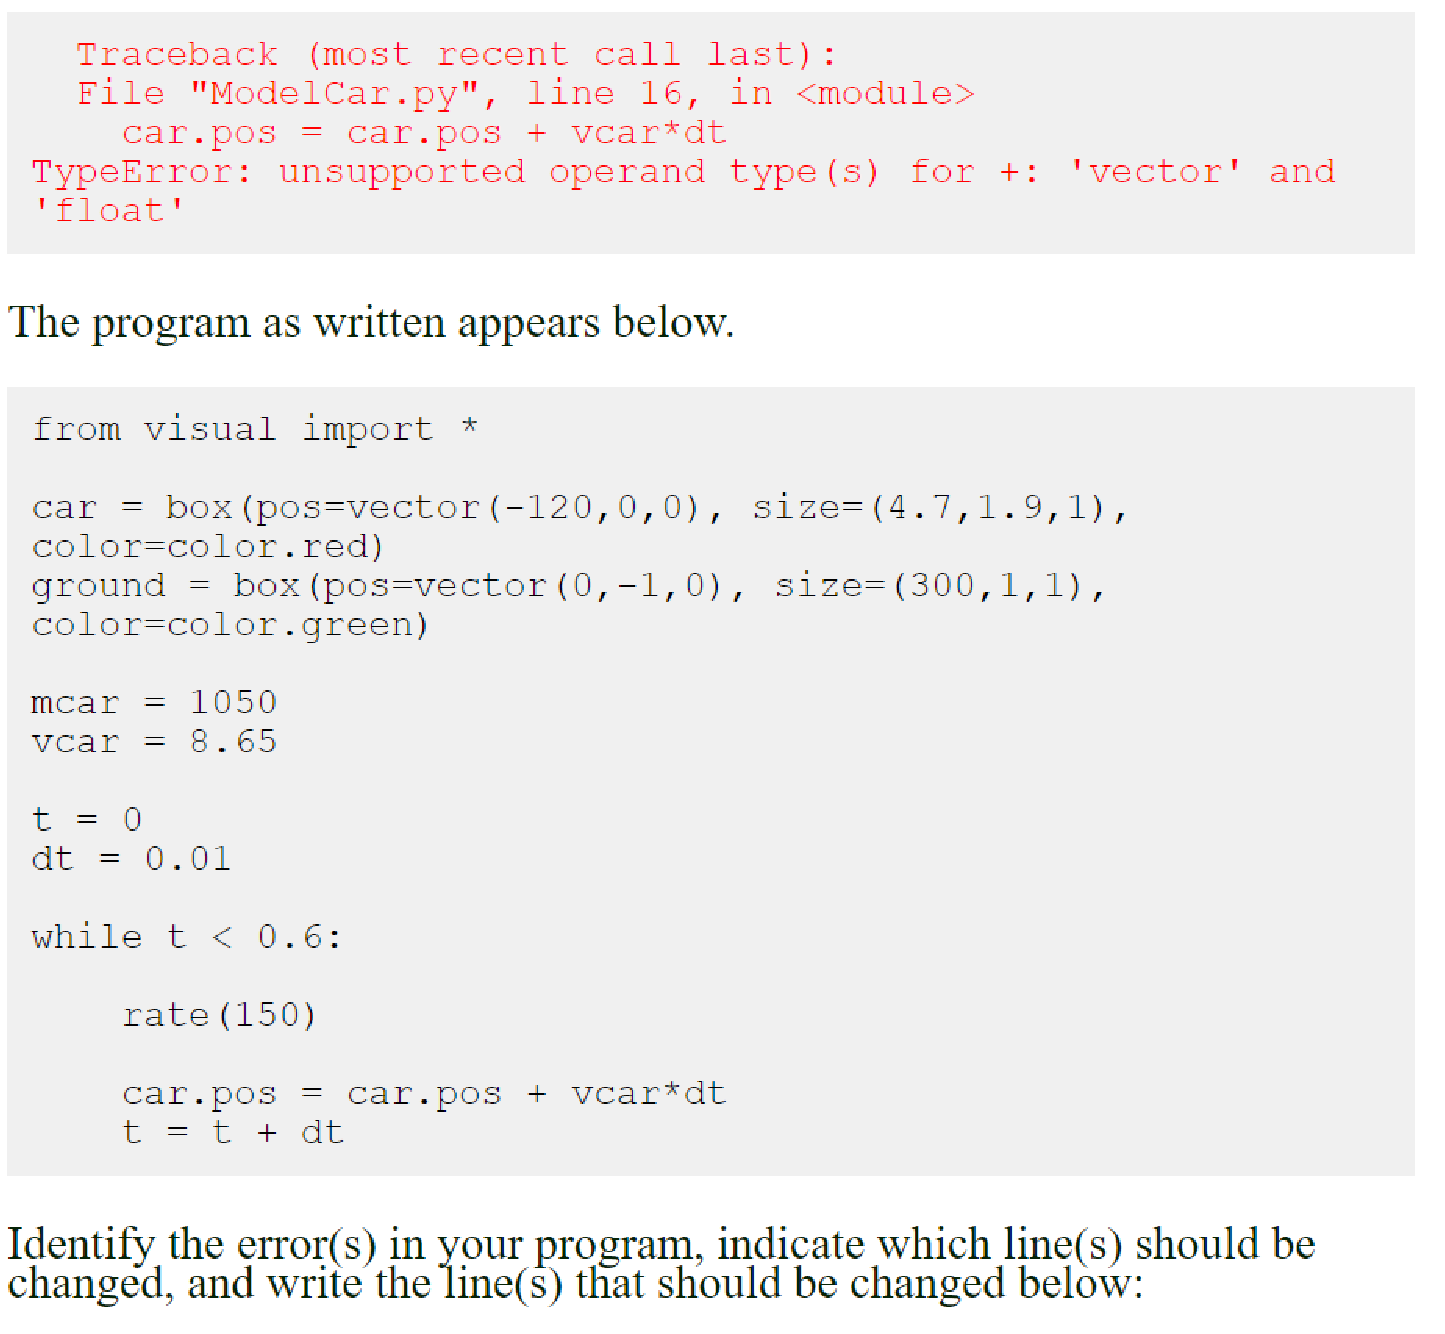
\includegraphics[scale=0.50]{images/CH3PostClassHomework.pdf}
\caption{A portion of a post-class homework question delivered in the third week of the course.  This question requires students to troubleshoot and debug the code.}\label{CH3:PostClassHomework}
\end{figure}

This type of problem helps to encourage students to identify, isolate, reproduce, and correct unexpected problems that arise while constructing computational models.  Ideally, it requires students to interpret the names given to the variables being used and verify that they are defined in a correct form.  Correct form means following one of the basic rules of algebra -- you cannot add a scalar and a vector.

%
%
%
%
%
%
%
%
%	MOTIVATION
%
%
%
%
%
%
%
%

\chapter{Motivation}\label{CH4:Motivation}

Aside from a general interest in introductory computational physics, it is important to understand the underlying motivation(s) for this thesis.  Sections from the following chapter, detailing some of those motivations, were published in the proceedings of the 2015 Physics Education Research Conference \cite{AAPT2016}, and is presented here with minor modifications from its appearance in publication. It was published with second and third authors Paul W. Irving and Marcos D. Caballero, respectively.

The process of identifying an interesting computational practice, described in Sec.~\ref{Sec:Debug}, was the earliest motivation for this study.  We found that it was extremely difficult to define and identify the particular practice of what we named ``physics debugging.''  Not only did the practice need to be clearly defined, it also needed to be clearly identified in the data.  This required a lot of in-depth qualitative analysis and inter-rater reliability, motivating our use of the Weintrop framework and the qualitative methods of Clarke et. al.

Additionally, as described in Sec.~\ref{Sec:Phenom}, we found that it was very difficult to understand the qualitatively different ways in which students experienced computational introductory physics.  This difficulty motivated a task analysis with a focus on identifying practices that the students were engaging in through in-class observation, as opposed to their experiences through out-of-class interviews.
  
\section{Debugging}\label{Sec:Debug}

In this section, we present a case study of a group of students immersed in this ${\rm P}^{3}$ environment solving a computational problem.  This problem requires the translation of a number of fundamental physics principles into computer code.  Our analysis consists of qualitative observations in an attempt to describe, rather than generalize, the computational interactions, debugging strategies, and learning opportunities unique to this novel environment.

\begin{figure}\centering
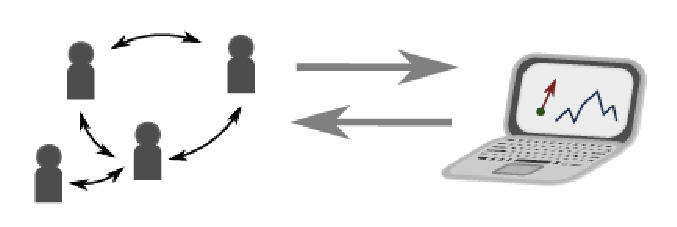
\includegraphics[scale=1]{./images/CH4Interactions.pdf}
\caption{Caption.}\label{CH4:Interactions}
\end{figure}

We focus this case study on the interactions between group and computer, illustrated in Fig.~\ref{CH4:Interactions}, to begin to understand the ways in which computation can influence learning.  Particularly, we are interested in the interactions occurring simultaneously with social exchanges of fundamental physics principles (FPPs) specific to the present task (e.g., discussing $d\mathbf{r}=\mathbf{v}\,dt$ on a motion task) and the display of desirable problem solving strategies (e.g., divide-and-conquer).  These group-computer interactions vary in form, from the more active process of sifting through lines of code, to the more passive process of observing a three-dimensional visual display.

One previously defined computational interaction that reinforces desirable strategies, borrowing from computer science education research, is the process of debugging \cite{Fitzgerald2008}.  Computer science defines debugging as a process that comes after testing \emph{syntactically} correct code where programmers ``find out exactly where the error is and how to fix it. \cite{McCauley2008}''  Given the generic nature of the application of computation in computer science environments (e.g., data sorting, poker statistics, or ``Hello, World!'' tasks), we expect to see unique strategies specific to a computational \emph{physics} environment.  Thus, we extend this notion of computer science debugging into a physics context to help uncover the strategies employed while groups of students debug \emph{fundamentally} correct code that produces unexpected physical results.

\subsection{Analysis}

In Fall 2014, ${\rm P}^{3}$ was run at Michigan State University in the Physics Department.  It was this first semester where we collected \emph{in situ} data using three sets of video camera, microphone, and laptop with screencasting software to document three different groups each week.  From the subset of this data containing computational problems, we \emph{purposefully sampled} a particularly interesting group in terms of their computational interactions, as identified by their instructor.  That is, we chose our case study not based on generalizability, but rather on the group's receptive and engaging nature with the project as an \emph{extreme case}.\cite{Flyvbjerg2006}

The project that the selected group worked on for this study consists of creating a computational model to simulate the geosynchronous orbit of a satellite around Earth.  In order to generate a simulation that produced the desired output, the group had to incorporate a position dependent Newtonian gravitational force and the update of momentum, using realistic numerical values.  The appropriate numerical values are Googleable, though instructors encouraged groups to solve for them analytically.

This study focuses on one group in the fourth week of class (the fourth computational problem seen) consisting of four individuals: Students A, B, C, and D.  The group had primary interaction with one assigned instructor.  Broadly, we see a 50/50 split on gender, with one ESL international student.  Student A had the most programming experience out of the group.  It is through the audiovisual and screencast documentation of this group's interaction with each other and with the technology available that we began our analysis.

To focus in on the group's successful physics debugging occurring over the $\SI{2}{\hour}$ class period, we needed to identify phases in time when the group had recognized and resolved a physics bug.  These two phases in time, \emph{bug recognition} and \emph{bug resolution} are the necessary limits on either side of the process of \emph{physics debugging}, as represented in Fig.~\ref{CH4:Strategies}.  We identified these two bounding phases at around $\SI{60(5)}{\minute}$ into the problem, and further examined the process of debugging in-between.  That is, we focused on the crucial moments surrounding the final modifications that took the code from producing unexpected output to expected output.

\begin{figure}\centering
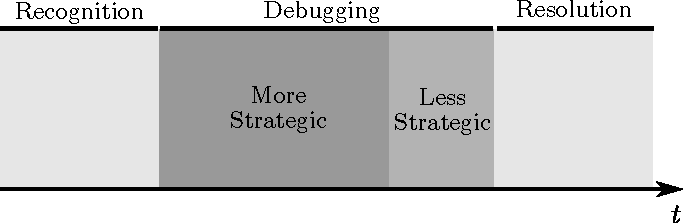
\includegraphics[scale=1]{./images/CH4Strategies.pdf}
\caption{The debugging process necessarily corresponds to a phase beset on either side by the phases of recognition and resolution.  Note the absence of a vertical scale, as the vertical separation merely acts to distinguish phases.}\label{CH4:Strategies}
\end{figure}

\subsubsection{Recognition}

At around 55 min into the problem, following an intervention from their instructor, the group began to indicate that they were at an impasse: \begin{description}
\SB We're stuck.
\SD Yeah...\end{description} The simulation clearly displayed the trajectory of the satellite falling into the Earth not the geostationary or bit they expected as observed on the screencast. This impasse was matched with an indication that they believed the FPPs necessary to model this real world phenomenon were incorporated successfully into the code:\begin{description}
\SB And it's gonna be something really dumb too.
\SA That's the thing like, I don't think it's a problem with our understanding of physics, it's a problem with our understanding of Python.\end{description}  Instead of attributing the unexpected output with a mistake in their understanding or encoding of FPPs, they instead seemed to place blame on the computational aspect of the task.

During this initial phase, we see a clear indication that the group has recognized a bug -- there is an unidentified error in the code, which must be found and fixed: \begin{description}
\SA I don't know what needs to change here...
\SD  I mean, that means we could have like anything wrong really.\end{description}  Although they have identified the existence of the bug, they still are not sure how to fix it -- this necessitates the
process of debugging.

\subsubsection{Physics debugging}

Within the previously identified phase of bug recognition, the group developed a clear and primary task: figure out exactly how to remove the bug. Eventually, following a little off-topic discussion, the group accepted that in order to produce a simulation that generates the correct output, they must once again delve into the code to check every line:\begin{description}
\SA ...I'm just trying to break it down as much as possible so that we can find any mistakes.\end{description}  In this way, the group began to not only deter mined the correctness of lines of code that have been added/modified, but also began to examine the relation ships between those lines.

For example, the group began by confirming the correctness of the form of one such line of code:\begin{description}
\SA Final momentum equals initial momentum
plus net force times delta t. True?
\SC Yeah...
\SB Yes.
\SA O.K. That's exactly what we have here. So this is not the problem. This is right.
\SD Yeah.\end{description}  That is, Student A i) read aloud and wrote down the
line of code $\vec{p}_{f} = \vec{p}_{i} + \vec{F}_{\rm net}*dt$ while the entire group confirmed on its correct form. This written line was then boxed, and was shortly followed up (ii) with a similar confirmation of the line $\vec{r}_{f} = \vec{r}_{i} + \vec{v}*dt$ that immediately
prompted (iii) the confirmation of $\vec{v} = \vec{p}/m$. Thus, not only do we see the group determining the correctness of added/modified lines of code as in (i)---(iii), we further see confirmation with the links between those lines. The confirmation of the link between the lines of code (i) and (ii), representing the incremental update of position and momentum in time, respectively, was evidenced not through the mere addition of the linking equation (iii) to the list of lines added, but further through the gestures exhibited by student A. Pointing at (iii), the $\vec{v}$ in (ii), and the $\vec{p}_{f}$ in (i), demonstrated that the group understood that without this linking equation (iii), the velocity used in (ii) would not reflect the time updated velocity by means of (i).

The group ran through these types of confirmations with FPPs rapidly over the span of a few minutes. Once the group had confirmed all the added/modified lines of code to their satisfaction, the discussion quieted down. The FPPs were winnowed from the discussion, and after a little more off-topic discussion we find them seeking help from the instructor:\begin{description}
\SD  Maybe we should just stare at him until he comes help us...\end{description} Suddenly, a haphazard change to the code:\begin{description}
\SA You know what, I'm gonna try something... \end{description} where Student A changed the order of magnitude of the initial momentum a few times. This modification even tually resulted in a simulation that produced the correct output.

\subsubsection{Resolution}

At about 65 min into the problem, Student A changed the order of magnitude of the momentum one final time, which produced something closer to the output that they expected: \begin{description}
\SA Oh wait... Oh god...
\SD Is it working?\end{description}  The satellite now elliptically orbited the Earth. This marks the end of the debugging phase and the beginning of the resolution phase the bug had successfully been found and remedied. Given that the only line of code modified to produce this change was the initial momentum, they began to rethink the problem:\begin{description}\SD I think that is the issue is that we don't have the initial momentum...
\SA ...momentum correct?\end{description}  That is to say, the group pursued the issue of determining the correct initial momentum with the added insight gained through debugging fundamentally correct VPython code.

\subsubsection{Strategies}

This case study has described two strategies (one more and one less strategic) employed by a group of students in a physics course where students develop computational models using VPython while negotiating meaning of fundamental physics principles. These strategies arose through the group's process of debugging a fundamentally correct program that modeled a geostationary orbit. The additional data we have collected around students' use of computation is rich, and further research is needed to advance the depth and breadth of our understanding of the myriad of ways in which students might debug computational models in physics courses.

\section{Phenomenography}\label{Sec:Phenom}

We also conducted a phenomenography in order to characterize the qualitatively different ways in which students were experiencing the problem.  In order fill the outcome space, we looked for the variation in students descriptions of what we called the ``critical'' components of the problem.  This was accomplished through post-class interviews where we followed a semi-structured protocol that was developed specifically for this case study.  Some of the very interesting results that can be generated from this type of analysis is presented in \cite{Hawkins2017}.

%
%
%
%
%
%
%
%
%	ANALYSIS
%
%
%
%
%
%
%
%

\chapter{Observations}\label{CH5:Observations}

Throughout our analysis in this thesis, we have made many different types of observations, and have used those observations to help answer our research questions (for example, see Sec.\ref{CH2:Thematic}).  Accordingly, it is important that we take some time to elaborate on the process of and results from those observations.  More specifically, in this chapter, we detail the method of our analysis (i.e., the data reduction, the coding process, and the inter-rater reliability) and illustrate the identification of three of the most frequent practices (i.e., troubleshooting and debugging, assessing computational models, and creating computational abstractions).

\section{Analysis}

Our full analysis involves different stages: first, the initial data was collected and subsequently reduced in order to provide a manageable set of data; next, an independent coding scheme was generated -- using the Weintrop framework from Sec.~\ref{CH2:Framework} -- to help identify computational practices; and finally, multiple inter-raters were used to ensure the reliability of the analysis.  Each of these three stages are detailed below.

\subsection{Data reduction}

Our total set or corpus of data consists of in-class video of nine groups of four individuals working.  Each group works on three computational problems (twenty-seven videos in total) that increase in difficulty/complexity as the semester progresses.  These computational problems, described in Sec.~\ref{CH3:Schedule}, require students to construct various computational force models in code.  Each week, the appropriate force model increases in complexity and generality.  Specifically, the first problem involves a constant zero force, the second problem involves a constant non-zero force, and the third problem involves a non-constant force.

In order to first reduce the corpus of our data to a more focused and manageable set, we payed attention to when students were making the most progress toward a solution.  The frequency of independent progress being made increased as the complexity of the problem increased (i.e., students made the most independent progress on constructing the Newtonian gravitational force model).  Here, we are defining ``independent progress'' as progress that is ultimately made by the group without any instructor intervention.  We believe this is due, in part, to their lack of prior programming experience coming into the course -- in other words, they progress quickly.  For example, on the first problem, many groups struggled with a basic calculation (while) loop.  By the time they see the third problem, they have already gained a little experience and are becoming accustomed to the norms of the course (e.g., their familiarity with the format, the programming environment, etc.).

Our initially reduced set of data consists of transcripts from in-class video (both side-view and overhead-view) of nine groups working on the Newtonian gravitational force problem from Sec.~\ref{CH3:SatelliteProblem}.  We also collected computer screencasts to capture exactly what students are doing when they type/click on their group laptop.  Following the suggestions of thematic analysis (see Sec.~\ref{CH2:Thematic}), we began with a full transcription of the in-class video to the best of our abilities.  Any inaudible sections are indicated, with long pauses being indicated by ellipses ($\ldots$).  To distinguish between unspoken actions (e.g., pointing to an equation) and inferences made by the primary researcher (e.g., a group referring to a previously used equation), we follow the convention of square brackets ($[\,]$) and curly brackets ($\{\,\}$), respectively.  For example, Fig.~\ref{CH5:Transcript} shows a portion of transcript highlighting these various indications.

\begin{figure}\centering
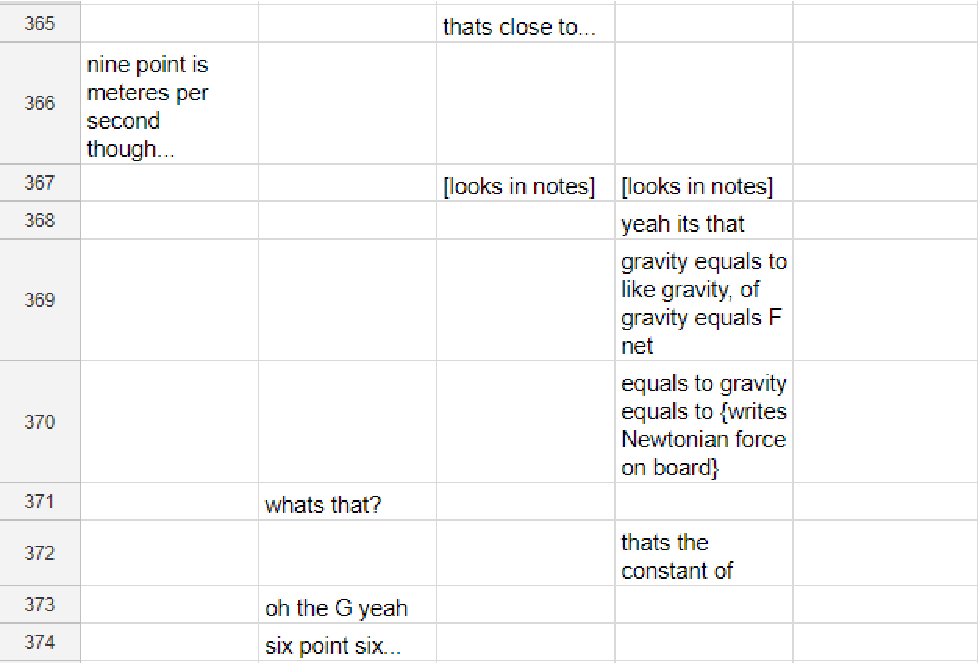
\includegraphics[scale=0.75]{./images/CH5Transcript.pdf}
\caption{A portion of transcript meant to highlight the indication of unspoken and inferred actions.  For example, line 367 shows this group looking in their notes for an equation.  The equation that they find is written down in line 370.}\label{CH5:Transcript}
\end{figure}

Once we had reduced our data corpus to a more manageable and focused set of nine transcripts, we continued our investigation into the computational practices students were engaging in.  Each transcript was read multiple times in order to generate a low-resolution but coherent picture of what each group was doing -- or at least, what each group was trying to do.  This type of ``familiarization'' with the data is a crucial step as outline by Braun et. al.  Ultimately, this low-resolution picture helped us to identify the off-topic and otherwise irrelevant discussion in order to remove those portions of the data from our analysis.

More specifically, each transcript was initially analyzed with an eye towards identifying discussion where students were i) solving the satellite problem and ii) using a computer (e.g., typing or reading through lines of a program).  All other discussion then could be considered off-topic and safely discarded.  For example, groups are often seen discussing homework for other classes that in no way relates to the Newtonian problem.  Similarly, groups can often be seen discussing recent social events (e.g., a concert).  This type of off-topic and otherwise irrelevant discussion, although important for the social cohesion of the group, can safely be discarded.  In this way, we further reduce our data set by about one quarter.  With each of nine transcript being about fifteen-hundred lines of speech/action, this translates to about ten-thousand lines of on-topic discussion for further analysis.

A closer analysis of this on-topic discussion is where we begin to more clearly define what computational practices look line within our data.  This closer analysis started with the search for a number of characteristics (as described in Sec.~\ref{CH2:Framework}), within the on-topic discussion.  For example, the key characteristics for the practice of troubleshooting and debugging are: i) to identify and isolate an unexpected error, ii) articulate how to reproduce the error, and iii) work to systematically correct it.  These characteristics, once identified, can be used to justify the classification of an excerpt as the computational practice of troubleshooting and debugging (recall that each computational practice may be indicative of the computational thinking as described in Sec.~\ref{CH2:Framework}).  This justification allows us to define the computational practices we see in our data.  A detailed account of this process of justification is described below, with applications to specific examples following in Sec.~\ref{CH5:Practices}.

\subsection{Coding process}\label{CH5:CodingProcess}

In order to justify the classification of an excerpt as a particular computational practice, we started by systematically coding our data.  This systematic coding process was applied to three streams of data: the side-view video, over-head video, and computer screencasts.  These three streams were then used to generate three types of rationale: rationale accordingly to the framework, rationale within an individual excerpt, and rationale beyond an individual excerpt.  These three types of rationale are described in detail below.

In terms of the framework, we identified the various characteristics that manifested themselves in the actions and speech of each group and compared them to the Weintrop framework.  Each practice, according to the framework, has any number (between one and seven) of related characteristics.  The more related characteristics that we see in an excerpt, the more confident we are in classifying that excerpt as a particular practice.  For example, ``identifying an unexpected error in code'' is one of the required characteristic of troubleshooting and debugging.  Similarly, ``working to systematically rectify the unexpected error'' is clearly a related but distinct characteristic.  The identification of either of these characteristics individually would be hinting at the practice of troubleshooting and debugging, but both of them simultaneously makes a stronger claim.  This type of rationale can be found in Column G of Fig.~\ref{CH5:Types}.

Within an individual excerpt, we are able to focus in on what each member of the group says and does as they work toward a clear and focused goal.  Any rationale of this type usually references line numbers pertaining to specific lines of speech/action within the excerpt that embodies the characteristic in question.  In this way, we closely tie our rationale and the framework to the data.  For example, a group might identify an unexpected error in their program and say: \begin{description}
\SC \textit{(756)} oh there it is \{the error message\}
\SB \textit{(757)} where?
\SC \textit{(758)} in the thing \{shell\} on the screen...
\end{description}  In this exchange, Student C has found the error message from the shell buried under a few other windows.  This error message is ultimately used by the group to track down the cause of the unexpected error.  In this way, we clearly see a group working to identify an unexpected error in our data.  This type of rationale can be found in Column H of Fig.~\ref{CH5:Types}.

Beyond each individual excerpt (i.e., looking at each transcript as a whole), we are able to generate a low-resolution picture that captures the overarching goals that each group is working toward.  This low-resolution picture helps us to contextualize each individual excerpt within the broader transcript.  There are many ways to contextualize a particular excerpt of data (e.g., in the context of the group, the classroom, the university, the state, etc.), and relating it to other excerpts is one of the most important.  For example, within an individual excerpt, a group might reference -- without defining -- an equation: \begin{description}
\SA \textit{(894)} should we try \textbf{that one} equation?
\SB \textit{(895)} yeah i think we should do that...
\SA \textit{(896)} okay
\SC \textit{(897)} yeah thats a good idea lets use that one
\end{description}  Using our low-resolution picture of the transcript as a whole, we can track back through time (often minutes, sometimes longer) to find out exactly what vague equation they are referencing: \begin{description}
\SC \textit{(120)} how about we use \textbf{the equation}...
\SC \textit{(121)} [writes G m M over r squared]
\SC \textit{(122)} ...and then multiplied by r hat
\SD \textit{(123)} i dunno...
\end{description}  Any rationale provided at this level usually references the number of another excerpt that provides the necessary additional information.  This level of rationale can be found in Column I of Fig.~\ref{CH5:Types}.

\begin{figure}\centering
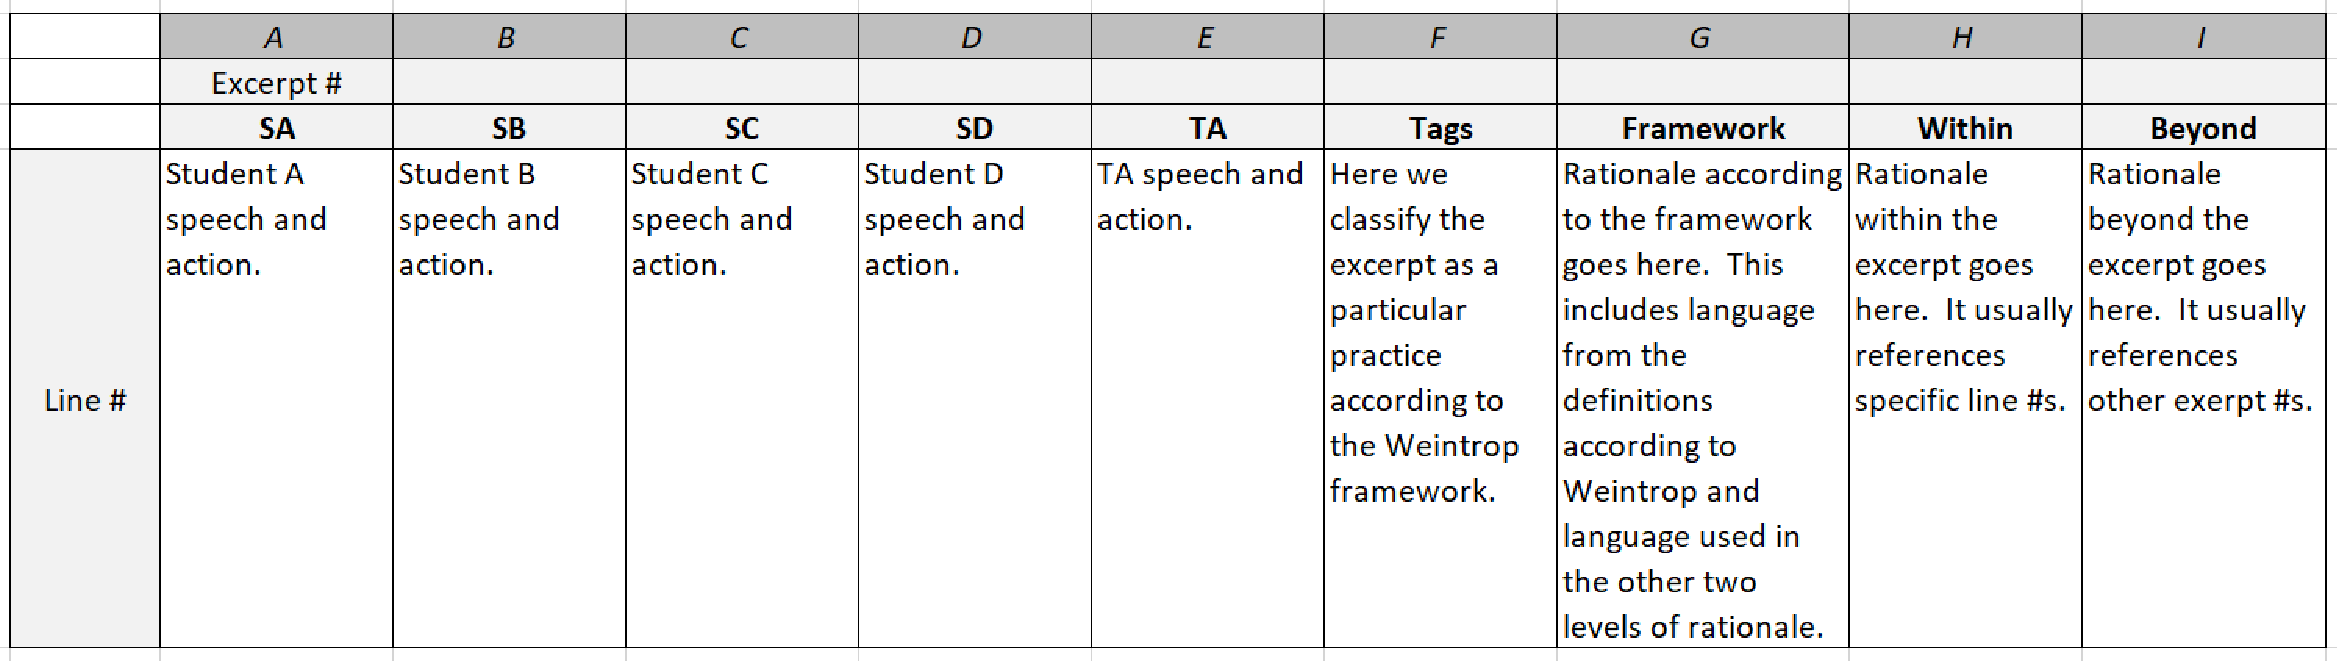
\includegraphics[scale=0.42]{./images/CH5Levels.pdf}
\caption{The template used for the coding process.  Each excerpt is numbered, each line of speech/action is numbered and attributed to an individual member of the group, and the three types of rationale are used to justify the classification of a particular practice.}\label{CH5:Types}
\end{figure}

This coding process was followed for nine groups to generate about five-hundred candidate excerpts, each excerpt having multiple practices, and each practice having the three types of rationale described above.  Each excerpt has anywhere from one to four possible practices identified with supporting rationale.  That equates to roughly three-thousand individual justifications that must be found within our data.

The three types of rationale described above, though not necessarily persuasive individually, when taken together can provide a reasonable justification for the classification of an excerpt as belonging to a particular computational practice: the rationale from the framework provides incomplete but guiding definitions, the rationale within an individual excerpt ties us closely to the data and the immediate actions that a group is taking, and the rationale beyond an individual excerpt helps to contextualize those immediate actions and speech.

\subsection{Inter-rater reliability}

In order to ensure not only reasonable, but also \textit{reliable} justifications for the classification of the various computational practices within our data, we followed an iterative process of inter-rater reliability.  One primary researcher was joined by three impartial inter-raters, ensuring a robust coding process and stronger claims through iterative critique and discussion.

\begin{figure}\centering
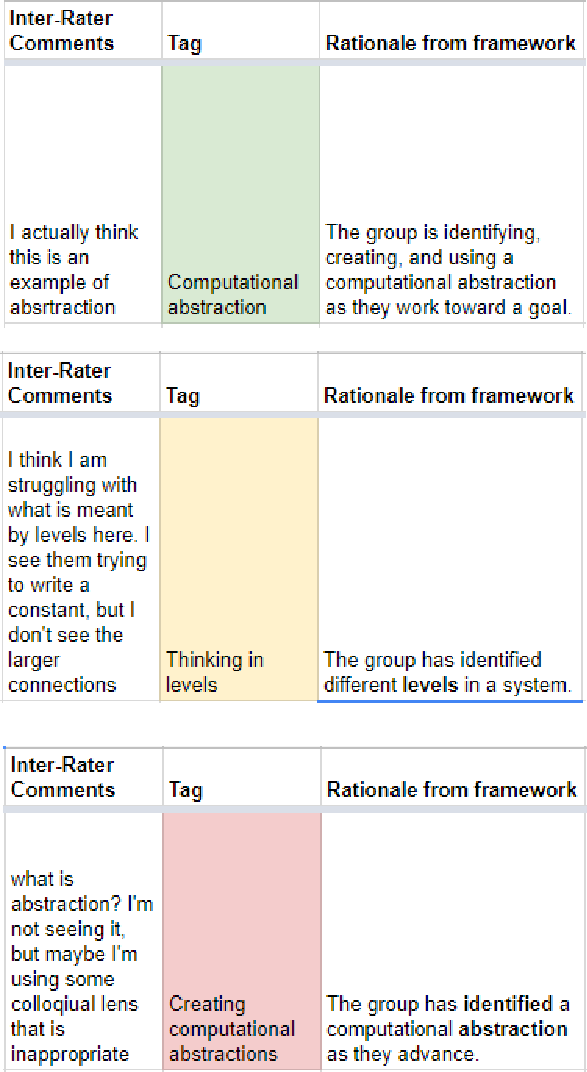
\includegraphics[scale=0.9]{./images/CH5LevelsofConfidence.pdf}
\caption{Examples of the three levels of confidence are shown in green (high), medium (yellow), and low (red) according to the supporting rationale from the framework.  Each inter-rater suggestion is used to modify or solidify the level of confidence given to a particular practice.}\label{CH5:LevelsofConfidence}
\end{figure}

Initially, the data was coded by the primary researcher, relying heavily on the Weintrop framework and the qualitative methods described in Ch.~\ref{CH2:Background}, to generate an initial set of rationale for each candidate excerpt.  This initial set of rationale for a particular excerpt, consisting of the three types of rationale described in the section above, was then taken as a whole to formulate an initial level of confidence: low, medium, or high.  Low confidence was usually given to excerpts containing only a few of the characteristics needed by a practice, or to excerpts where the identification of an individual characteristic was in serious question.  Medium confidence was given to excerpts containing most of the characteristics required by a practice, or to excerpts where the identification of individual characteristics was probable.  High confidence was given to excerpts containing all of the required characteristics for a practice, or to excerpts where the identification of each individual characteristic was self-evident.  Examples of excerpts belonging to these different levels of confidence are shown in Fig.~\ref{CH5:LevelsofConfidence}.

\begin{figure}\centering
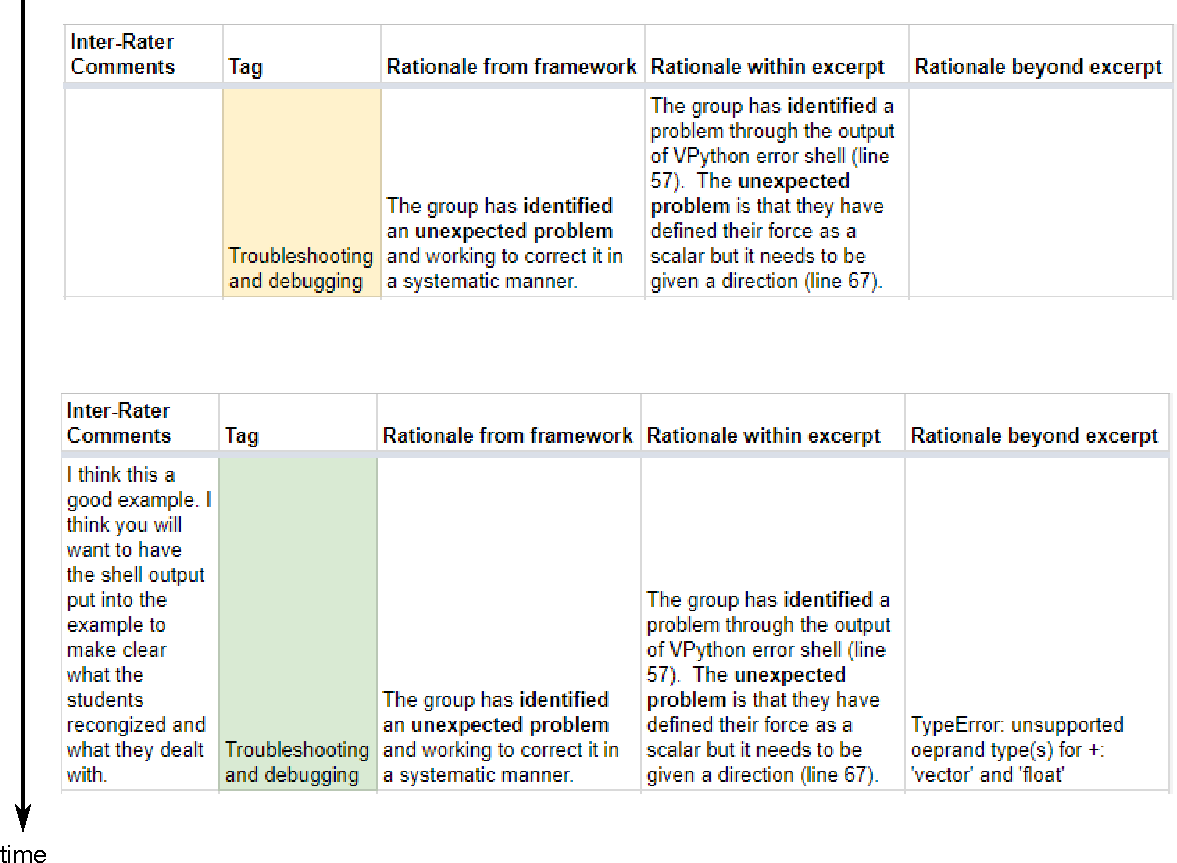
\includegraphics[scale=0.65]{./images/CH5Reliability.pdf}
\caption{The initial rationale generated for an excerpt along with inter-rater suggestions and subsequent modification.  With the addition of some requested information, the strength of the rationale was improved and the confidence was promoted from medium to high.}\label{CH5:Reliability}
\end{figure}

A subset of the data containing a variety of computational practices and levels of confidence was then shared with multiple inter-raters.  Each inter-rater subsequently tested the strength of our initial claims through discussion by asking questions and making suggestions.  These suggestions, once mutually agreed upon, were incorporated into the rationale.  For example, Fig.~\ref{CH5:Reliability} shows one inter-rater asking a clarification question as to what the verbatim output of the shell in a particular excerpt was.  The answer to this clarification question, though no obvious given the initial rationale, proves to be relevant and necessary to the strength of the rationale.  Accordingly, this inter-rater suggests that this additional information be added to the rationale to improve confidence.  This process of generating reliability through asking questions and making suggestions was followed iteratively to further strengthen each claim.

\section{Computational practices}\label{CH5:Practices}

By analyzing all of the data with the methods described above, we have confidently identified a number of practices that show up in our data.  These practices and their frequencies within our data are summarized in Fig.~\ref{CH5:DensityPlot}.  In total, we identified roughly 250 occurrences of individual practices, with some practices occurring frequently and some occurring never.  The most frequent practices, though found within our \textit{unique} data, can be expected to arise just as frequently in sufficiently similar classrooms and deserve a fair amount of attention.

\begin{figure}\centering
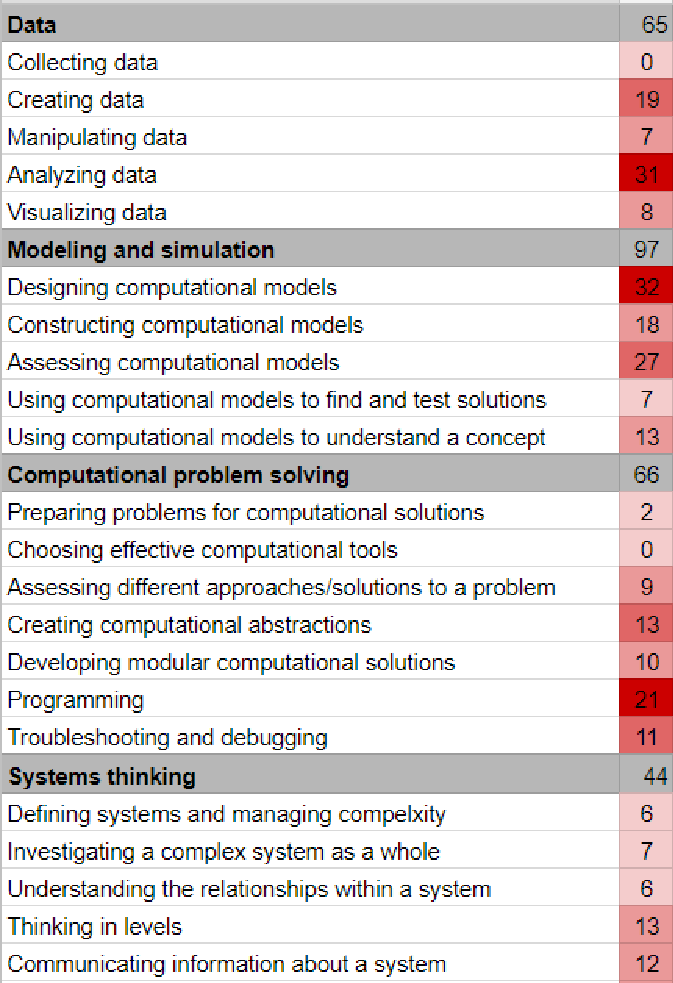
\includegraphics[scale=0.65]{./images/CH5DensityPlot.pdf}
\caption{The frequency of each practice that was found within our unique data set.}\label{CH5:DensityPlot}
\end{figure}

The remainder of this section provides concrete examples of the most frequent computational practices that we found in our data.  These practices are (in no particular order): creating and analyzing data within the data practices; designing, constructing, and assessing computational models within the modeling and simulation practices; programming, creating abstractions, and troubleshooting and debugging in the computational problem solving practices; and thinking in levels and communicating information within the systems thinking practices.

The other less frequent practices, though not the focus here, are still of great research interest.  Some of these less frequent but nonetheless important computational practices can be found in the Appendix.

%
%
%
%
%
%
%
%
%	CREATING DATA
%
%
%
%
%
%
%
%

\subsection{Creating data}

The computational practice of creating data, as defined by Weintrop et. al, involves the generation (as opposed to collection) of computer data while ``investigating phenomena that cannot be easily observed or measured or that are more theoretical in nature.''  This type of data creation frequently arises in physics and engineering given the infeasibility of data collection in many realistic situations.  For example, complex computer models can be used to generate data that can be used to optimize launch conditions for satellites and manned rockets when real-world collection of data is too costly or dangerous.  The fundamental characteristics associated with this practice are: i) defining a computational procedure that creates data and ii) using that procedure/data to advance their goals.

\begin{table}[t]
\begin{tabular}{r|p{0.8\textwidth}}
Characteristic & Qualities \\\hline\hline
Automating & The data that is being created should be done so in an automatic or algorithmic manner.  For example, an Euler-Cromer style integration is frequently used to generate large sets of numerical data representing various physical phenomena in time.\\
Advancing & Each group should ultimately be advancing their understanding of a phenomenon as they work to complete their goals.\\
\end{tabular}\caption{The characteristics and associated qualities pertaining to the computational practice of creating data.}
\end{table}

Consider Excerpt 9 from Group H.  Over the course of two hours, this group can be seen ensuring that their MWP will dynamically update the position of the satellite.  This entails ensuring that the momentum of the satellite will also dynamically update.  Accordingly, the group works to construct a computational algorithm that will automatically create sets of data representing the positions and momenta of the satellite over time.  These sets of data are then ultimately used to create visualizations which help them to advance their understanding of the satellite's motion.

Early on, the group can be seen considering changing the initial position (line 199) of the satellite to what they calculated from the previous problem:
\begin{description}		
\SD \textit{(195)} So, it's mostly just {trying} to figure out how to get it {the satellite} to display {an orbit}...
\SA \textit{(196)} Yeah, it is.	
\SC \textit{(197)} Wait, we have to change the position, don't we?	
\SB \textit{(198)} I think {the initial} position stays there, we have to update position though...
\SC \textit{(199)} Yeah, we have to change {the initial} position to what we found... it was this far away, you know?	
\SA \textit{(200)} Yeah.		
\SB \textit{(201)} Yeah.
\SA \textit{(202)} Which was... four point four two times ten to the seven.
\SB \textit{(203)} Four point two... [codes]
\end{description}  They seem to make the distinction between changing the initial position of the satellite and changing the way that the position updates over time (line 198).  This is an important distinction because each change involves vastly different amounts work to accomplish.

Eventually they propose an Euler-Cromer style algorithm to update the position of the satellite (line 222) in terms of its momentum, mass, and time:
\begin{description}
\SB \textit{(214)} Hey it moves... that's exciting... that doesn't do anything though.
\SA \textit{(215)} It just made it... far.
\SA \textit{(216)} Okay, and then the velocity...
\SB \textit{(217)} Alright...
\SB \textit{(218)} Okay, so we have to add it's {new} position.
\SA \textit{(219)} But it has to update its position every time...
\SB \textit{(220)} Right.
\SA \textit{(221)} So we have to make it update.
\SB \textit{(222)} Satellite position plus momentum of the satellite...
\SA \textit{(223)} Over the mass?			
\SB \textit{(224)} Times the change in time... yeah so its, yeah.
\SB \textit{(225)} But the momentum is always changing...
\end{description}  Although the group has clearly laid out the way that the position of the satellite will need to change (line 222), they have raised another issue in terms of the momentum of the satellite (line 225).  In other words, they have defined a procedure to calculate the positions of the satellite, but still need to define a procedure to calculate the momenta.

As the group works toward defining a procedure to change the momentum of the satellite over time, they recall the concept of both iterative prediction (line 684) from the notes and Newton's second law (line 695):
\begin{description}
\SB \textit{(681)} So we gotta figure out how to change the momentum in there {the code}.
\SB \textit{(682)} What was the equation from last week?		
\SA \textit{(683)} Umm... F grav... no.
\SD \textit{(684)} What about using iterative prediction for like future positions?
\SD \textit{(686)} Right?
\SC \textit{(687)} The change in momentum would be the net force times...	
\SB \textit{(688)} Because the force is mass times acceleration...
\SC \textit{(689)} That would be it, yeah.
\SB \textit{(690)} So integrate that.
\SC \textit{(692)} Changing momentum is force times change in time...
\SB \textit{(693)} Oh, there we go, nice.
\SA \textit{(694)} Wait what is it?
\SB \textit{(695)} The change in momentum is the net force times change in time.
\end{description}  With these two procedures defined, their MWP is ready to dynamically update the position, momentum, and eventually the force of the satellite.

To summarize, the group can be seen \textit{automating} the generation of sets of data representing the position and momentum of the satellite over time.  Further, with these sets of data, the group is ultimately \textit{advancing} their understanding of the concept of predictive motion and their progress toward constructing a generalizable simulation of orbital motion.  Given the identification of these two characteristics, this excerpt is best classified as the computational practice of creating data.

%
%
%
%
%
%
%
%
%	ANALYZING DATA
%
%
%
%
%
%
%
%

\subsection{Analyzing data}

The computational practice of analyzing data, as defined by Weintrop et. al, usually involves large sets of data (that have either been created or collected) where groups are ``looking for patterns or anomalies, defining rules to categorize, and identifying trends and correlations.''  This type of analysis shows up frequently within the field of physics, especially given the computational nature of many (if not most) modern investigations.  For example, extremely large sets of data are generated while investigating the formation and evolution of galaxies in our solar system.  Being able to effectively analyze a large set of data is a crucial skill within many interdisciplinary fields.  The fundamental characteristics associated with this computational practice are: i) a process of analysis and ii) a claim being made based on that analysis.

\begin{table}
\begin{tabular}{r|p{0.8\textwidth}}
Characteristic & Qualities \\\hline\hline
Analyzing & This is a broad term that usually involves at least one of many acts.  For example, sorting a set of data into different categories, looking for trends or patterns within a given set, looking for correlations between multiple sets, and/or identifying outliers and anomalies are all captured under the umbrella of analysis.\\
Claiming & The information (e.g., a pattern or an anomaly) gathered from the analysis of a set of data should ultimately be used to make some claim.  This characteristic, though an important one, is not necessarily required for a group to be analyzing data.\\
\end{tabular}\caption{The characteristics and associated qualities pertaining to the computational practice of analyzing data.}
\end{table}

Consider Excerpt 35 from Group H.  Overall, this group can be seen engaging in the process of analysis of a set of data that represents the net force acting on the satellite, and making a claim based on the results of that analysis.  The particular process of analysis observed here involves both categorization and patterning.  The categories involved here are: a) large numbers and b) vectors.  The pattern that the group recognizes is that the net force is a time-dependent force.

Previous to the beginning of this excerpt, the group added a print statement (i.e., \texttt{print(Fnet)}) into their calculation loop to print off the numerical values for the components of the net force acting on the satellite over time.  Presumably, they do this to check their model is producing the expected values:  \begin{description}
\SD \textit{(1330)} How many times does this {calculation loop} run through?
\SB \textit{(1331)} A lot...		
\SD \textit{(1332)} Yeah.. a lot [looking at output].
\SB \textit{(1333)} However many seconds are in a day.
\SA \textit{(1334)} Eighty six thousand.
\SD \textit{(1335)} Wow...
\SB \textit{(1336)} Yeah doing it line by line is not gonna be easy.
\end{description}  With this print statement, they are creating a large set of data (line 1332) that can be further analyzed.

The group confirms that their print statement is displaying a large set of data that represents the net force on the satellite (line 1338).  At the same time, they begin to categorize their data and look for trends:
\begin{description}
\SD \textit{(1337)} It's not showing it {the satellite} because I think the scale is too small.
\SD \textit{(1338)} But its outputting all of it {the forces}, and it is...
\SD \textit{(1339)} It's changing too I think.
\SB \textit{(1340)} How big are they?		
\SB \textit{(1341)} I'm assuming were talking about F grav...
\SC \textit{(1342)} Yeah, it is big.
\end{description}  One trend that the group explicitly states (line 1339) is that the values in the set are non-constant in time.  Similarly, one category that this group implicitly places this set in (line 1342) is that of having a large order of magnitude -- which is expected given the type of force.

Mistakenly, the group suggests that the pattern they have recognized is not the expected or desired one.  In other words, they suggest that the set of data should be constant in time (line 1343):
\begin{description}
\SB \textit{(1343)} Uhh... I don't think its supposed to be changing.
\SB \textit{(1344)} Not a good sign.
\SB \textit{(1345)} Do we have it as a vector or a scalar right now?
\SD \textit{(1346)} Right now we have it as a vector.
\end{description}  Additionally, the group further categorizes the set of data (line 1346) as being a collection of vectors as opposed to scalars.

After letting the program run for a fair amount of time, they decide that they have gotten everything that they need for their analysis and terminate the program:
\begin{description}
\SD \textit{(1347)} Well it has run through about five hundred times now.
\SB \textit{(1348)} No maybe you should tell it not to print out the values.
\SB \textit{(1349)} So stop it...
\SD \textit{(1350)} That's a good point.
\SB \textit{(1351)} Tell it to stop printing out every single value.
\end{description}  Although this set of data is rather large (around five hundred data points by the time of termination), analysis can also be performed on individual numerical values.  However, this type of individual analysis is better described by the practice of assessing a computational model.

To summarize, this group can be seen \textit{analyzing} a set of data by identifying trends in the data, breaking the data up into different categories, and making claims based on the results of the analysis.  The trend observed here is that the data changes over time, and the data were placed in the categories of being large and also being vectors.  Additionally, the group can be seen (mistakenly) \text{claiming} that the data should not be changing.  Given this process of analysis and the claim being made, this excerpt is thought to illustrate the computational practice of analyzing data.

%
%
%
%
%
%
%
%
%	DESIGNING MODELS
%
%
%
%
%
%
%
%

\subsection{Designing models}

The computational practice of designing computational models, as defined by Weintrop et. al, involves the process of making ``technological, methodological, and conceptual decisions.''  These types of decisions are frequently dealt with in the STEM discipline given the complexity of modern scientific endeavors.  Scientific rigor and sound methodology must be utilized while using powerful tools at the forefront of technology (i.e., computation) to investigate modern phenomena.  At the same time, developing a deep conceptual understanding of the models and the phenomena that they represent is playing an increasingly important role in the sharing and communication of scientific information.  The fundamental characteristics associated with this computational practice are: i) defining the components of a model, ii) describing how the components of a model interact, and iii) articulating what data/conclusions cam be produced/drawn by the model.

\begin{table}
\begin{tabular}{r|p{0.8\textwidth}}
Characteristic & Qualities \\\hline\hline
Separating & Each individual component of a model must be separately defined in code.  For example, the mass and velocity of an object can be separately defined and used together to construct the momentum of the object.\\
Relating & The group must describe the way that the individual components interact to model a phenomenon.  This interaction usually mirrors an equation/relationship that they have seen in the notes.  For example, the momentum of an object is linearly proportional to not only the mass but also the velocity and can be used to calculate the position over time.\\
Predicting & The group must articulate what information their model will provide them, and use that information to make predications about the time evolution of a phenomenon given initial conditions.  For example, a force model can generate the various values of the force acting on an object at different positions in time.  This set of data can then be used to make predictions about the motion of the object.\\
\end{tabular}\caption{The characteristics and associated qualities pertaining to the computational practice of designing a computational model.}
\end{table}

Consider Excerpt 12 from Group G.  Overall, the group can be seen designing a model that can be used to calculate the position of the satellite over time.  This model involves the definition of the mass, position, velocity, momentum, and net force as the individual components that interact with time to integrate Newton's equations of motion.  Specifically, they focus on the way that the momentum interacts with the mass and velocity (i.e., $\vec{p}=m\vec{v}$) as well as the way that this momentum is used (along with the force) to calculate the position of the satellite over time (i.e., through the Euler-Cromer equations of $\vec{p}_{\rm new}=\vec{p}_{\rm old}+\vec{F}_{\rm net}dt$ and $\vec{r}_{\rm new}=\vec{r}_{\rm old}+(\vec{p}/m)dt$).

The group begins by recalling an equation (line 350) for the momentum of an object in terms of the mass and velocity of the object and begin to define them code: \begin{description}
\SA \textit{(350)} What's the equation for momentum?	
\SB \textit{(351)} Mass times velocity [looking in notes].
\SA \textit{(352)} Okay, so we have to add velocity \{in the code\}... We have the mass, we just fixed the mass...
\SB \textit{(353)} Right...
\SC \textit{(354)} So the mass...	
\SA \textit{(355)} We \{need to\} add the velocity, which we solved \{last time\} to be... uhh... thirty... err three thousand seventy one.
\SB \textit{(356)} What?		
\SA \textit{(357)} I said we add the velocity which we found to be three thousand seventy one.\end{description}  They have identified (line 352) that the mass of the satellite is already defined in their program and they have modified it so that it reflects the realistic value provided in the problem statement.  Next, they begin to define the velocity (line 355) of the satellite in terms of the numerical value that they calculated from the previous day's (related) problem.  In this way, the group is defining some of the individual components of the model representing the momentum and position of the satellite over time.

However, before getting too far, the group expresses concern about the fact that their program does not allow for the analysis of elliptical orbits.  In other words, they need the velocity of the satellite to change (line 358) over time:  \begin{description}
\SB \textit{(358)} I think in that thing \{the problem statement\} it said we have to do it elliptical too.
\SB \textit{(359)} Which would change the velocity.		
\SB \textit{(360)} So we have to figure out... we gotta write the entire \{Euler-Cromer\} equation in there how the velocity changes.
\SA \textit{(361)} Hold on...
\SB \textit{(362)} Yeah that's gonna be annoying.		
\SB \textit{(363)} Yeah, but the velocity has to change.\end{description}  Although they have defined the correct mass and initial velocity of the satellite, they have not yet related them to momentum.  The momentum is what shoes up in the Euler-Cromer equations to integrate the force into the position of the satellite.

A little later, they begin to describe the algorithm that utilizes the momentum to ensure that the velocity of the satellite will constantly and correctly change (line 752) over time so that they can investigate elliptical orbits: \begin{description}
\SD \textit{(750)} Then we have to update the momentum of the system with p final equals p initial plus F net times delta t.
\SD \textit{(751)} Or r final, which is for the position, equals r initial plus v average times delta t.
\SD \textit{(752)} So one updates the momentum and one updates the position.
\end{description}  This algorithm involves (line 750) the momentum of the satellite being changed by a force and its position being changed by its new momentum divided by its mass.  It seem as though they have correctly made the connection that their momentum divided by the mass is what gives them the average velocity as their code shows \texttt{sat.pos = sat.pos + (psat/msat)*dt} yet they mention the velocity and not the momentum (line 751).

To summarize, the group runs into an issue where the position of their satellite in not correctly being calculated over time.  This issue is ultimately due to the fact that the mass and the velocity of the satellite (both separately defined in code) were not being used to calculate the corresponding momentum (which is then used to calculate the new position).  However, once the momentum of the satellite is correctly defined in terms of its mass and velocity, it then correctly produces a set of data that can predict the position of the satellite for elliptical orbits.  That is, the group has \textit{separately} defined the mass, position, velocity, momentum, force, and time of the satellite as six individual components in their model of motion.  Further, they have described the way that these individual components \textit{relate} through of a process of Euler-Cromer style integration.  Finally, they have articulated that their model will be able to \textit{predict} the values for the velocity of the satellite over time which are then used to ultimately calculate the positions of the satellite for various initial conditions (i.e., elliptical orbits).  Given these characteristics that we have identified, this excerpt illustrates the computational practice of designing a computational model.

%
%
%
%
%
%
%
%
%	ASSESSING MODELS
%
%
%
%
%
%
%
%

\subsection{Assessing models}

The computational practice of assessing a computational model, as defined by Weintrop et. al, involves ``understanding how the model relates to the phenomenon being represented.''  This is a crucial step in the process of modeling -- without an assessment of the validity and meaning of the results (i.e., without a deep understanding), the model is almost certainly useless.  The fundamental characteristics associated with this crucial computational practice are: i) raising issues with the model and ii) identifying assumptions built into it.

\begin{table}
\begin{tabular}{r|p{0.8\textwidth}}
Characteristic & Qualities \\\hline\hline
Assuming & In designing a computational model, certain assumptions are invariably taken into account.  These assumptions -- regardless of how appropriate -- should be identified and clearly articulated by the group.  For example, the assumption that the satellite will be traveling in a circular orbit, although a poor one, is an assumption.\\
Validating & During the design and construction of a computational model, issues or threats to its validity are often raised.  For example, the fact that a particular model of motion cannot handle elliptical orbits is a threat to its generalizability or validity.\\
\end{tabular}\caption{The characteristics and associated qualities pertaining to the computational practice of assessing a computational model.}
\end{table}

Consider Excerpt 9 of Group C.  Generally speaking, the group can be seen working to incorporate a gravitational force into their code.  Early on, they recognize that their code is missing the net force on the satellite, and subsequently spend about thirty minutes deciding on if and how they should should incorporate a gravitational force.  Eventually they come a conclusion after assessing a couple of different options (i.e., a Newtonian or a local gravitational force).

At about 10 minutes in, the group considers what happens to the initial momentum as the program runs (line 256):
\begin{description}
\SA \textit{(253)} Umm...
\SB	\textit{(254)} Okay.
\SA \textit{(255)} So that's our initial momentum.			
\SA \textit{(256)} And then what happens...			
\SD \textit{(257)} And the...
\SA \textit{(258)} We need, we have it...		
\SA \textit{(259)} The net force equation is what's [inaudible]...
\SD \textit{(260)} Yeah, the net force equals to like gravity, right?\end{description}  Obviously the group is concerned with the state of the net force equation (line 259), and a proposal is made to set the net force equal some sort of gravitational force (line 260).  This is the beginning of an assumption that the group is making about their model (i.e., that it is a Newtonian gravitational force acting on the satellite as opposed to a local gravitational force).

They continue to discuss the gravitational force that they plan to incorporate into their code.  Specifically they wonder what numerical value they should be using (line 262), and Student A suggests using the local gravitational constant ($g=\SI{9.81}{\meter\per\second\squared}$):
\begin{description}
\SD \textit{(261)} So we just need to like plug in the value of gravity right?
\SA \textit{(262)} Yeah... but what's the value that we need?
\SA \textit{(263)} Because we have um... we have um... we have...
\SA \textit{(264)} Mass in kilograms and we have {the radius of orbit in} kilometers, obviously we all know like nine point eight number...
\SC \textit{(265)} That's close to {the surface of the Earth}...	
\SA \textit{(266)} Nine point is meters per second though.\end{description}  However, Student C recognizes that their satellite is not really that close to the surface of the Earth (line 265), and that the local gravitational constant really only applies there.  In other words, the group can be seen validating their computational model.

Eventually, the group does decide on a particular gravitational force to use (line 270):
\begin{description}		
\SC \textit{(267)} [looks in notes]
\SD \textit{(268)} Yeah it's that [points to equation].
\SD \textit{(269)} Gravity equals to like gravity, of gravity equals F net...
\SD \textit{(270)} Equals to gravity equals to {writes Newtonian force on board}...
\SB	\textit{(271)} What's that?		
\SD \textit{(272)} That's the constant of...
\SB	\textit{(273)} Oh the G yeah.		
\SB	\textit{(274)} Six point six...\end{description}  This force involves the universal gravitational constant ($G=\SI{6.61E-11}{\newton\meter\squared\per\kilo\gram\squared}$) which they clearly state (line 273).  Again, the group has validated their net force model by assesing the location of the satellite and the required gravitational constant.

Before getting to far, the group takes some time to clearly articulate an assumption (line 275) built into their code:
\begin{description}
\SA \textit{(275)} Sorry i just wanted to write here that we're making an assumption [writes on WB].
\SD \textit{(276)} Yes.
\SD \textit{(277)} F net equals to gravity.
\SD \textit{(278)} Yes.
\SD \textit{(279)} Equals to...
\SA \textit{(280)} I just did that [adding an E] to show that that's of the Earth.
\SA \textit{(281)} Does everyone agree that this is an assumption?	
\SC \textit{(282)} Yeah.
\end{description}  The fact that the only force acting on the satellite is a gravitational force, and the fact that the gravitational force should be of a Newtonian form, are really just assumptions made by the group at this point.  The group specifically takes the time to articulate and agree upon this assumption.

To summarize, the excerpt demonstrates two fundamental characteristics: the group is \textit{validating} their model when they compare which gravitational constant they should be using, and the group is \textit{assuming} things about their model when they say that the net force equals the Newtonian gravitational force.  Given these two characteristics, we feel confident in categorizing this excerpt as a strong illustration of the computational practice of assessing a computational model.

%
%
%
%
%
%
%
%
%	CREATING ABSTRACTIONS
%
%
%
%
%
%
%
%

\subsection{Creating abstractions}

The computational practice of creating abstractions, as defined by Weintrop et. al, requires ``the ability to conceptualize and then represent an idea or a process in more general terms.''  This ability show up frequently in the STEM domains -- especially within introductory computational physics.  The two fundamental characteristics of this computational practice are: i) conceptualizing an idea and ii) representing it in more general terms.  These two characteristics, if confidently observed within an excerpt, would serve to classify that excerpt as the computational practice of creating computational abstractions.

\begin{table}
\begin{tabular}{r|p{0.8\textwidth}}
Characteristic & Qualities \\\hline\hline
Conceptualizing & There needs to be some concept that a group is focusing on.  Concepts usually range from individual physical quantities to more complicated physical relationships.\\
Representing & A particular concept should be represented mathematically.  This process of representation usually involves translating a mathematical equation from the notes into a more general computer function.
\end{tabular}\caption{The characteristics and associated qualities pertaining to the computational practice of creating computational abstractions.}
\end{table}

Consider Excerpt 13 from Group D in the following analysis.  Overall, the group can be seen giving their net force a direction through the use of a unit vector ($\hat{r}$).  They first recognize that their force needs to be a vector, and propose an equation to use that specifically involves a direction ($\vec{F}\propto\hat{r}/r^{2}$).  Once they have their equation to work with, they begin to discuss how they can define it as a general function.  In other words, the group can be seen \textit{conceptualizing} and \textit{representing} an idea in general terms.

They start by looking for an equation that they can use to try to calculate the net force on the satellite: \begin{description}
\SA \textit{(108)} [calculating the magnitude of the force on his calculator]
\SC \textit{(109)} Yeah just try that one {equation} first.		
\SC \textit{(110)} If that's not gonna work, then \{I\} think \{the\} other...
\SD \textit{(111)} But the direction of F is \{a vector\}...	
\SD \textit{(112)} So we need to turn the r into a vector.
\SC \textit{(113)} I think we should...		
\SD \textit{(114)} [writes force equation with $\hat{r}$]
\end{description}  Here the group can be seen deciding (or at least suggesting in line 109) that the computational force model that they are using will need to take a direction into account (i.e., it needs to be a vector).  This equation, $\vec{F}\propto\hat{r}/r^{2}$ (retrieved from their notes), is written down on the WB.  Notice that it involves using $\hat{r}$ to give the force a direction.  This unit vector is the computational abstraction that the group identifies and ultimately begins to construct in their program.  This abstraction helps them to work toward their goal of constructing the non-constant Newtonian gravitational force on the satellite.

Once the unit vector ($\hat{r}$) has been identified as a computational abstraction, they begin its creation in code:\begin{description}
\SD \textit{(115)} So just put the r value, vector value...
\SD \textit{(116)} Just put this [points to r hat] uhh function...
\SB \textit{(117)} As a parameter?			
\SD \textit{(118)} Just give the \textbf{computer a function} so we don't have to calculate F {like SA is doing}.	
\SB \textit{(119)} That's a good idea.
\end{description} Although they are clearly focusing on the concept of the direction of the Newtonian gravitational force, they are a little stuck on how to actually go about creating it.  However, they at least know that they want it to be a function (line 118) rather than just a constant numerical value.  Presumably, this is because they know that the numerical values will need to change in time (line 271):\begin{description}
\SD \textit{(269)} No I mean this is the distance... and it has a direction...	
\SB \textit{(270)} So it's a vector.
\SD \textit{(271)} Yeah this {the position of the satellite} is a vector.
\SD \textit{(272)} Change with time...
\SC \textit{(273)} Yeah I'm talk about the very beginning with the D... here [points to WB].
\SB \textit{(274)} So the D is the radius...
\end{description}

To summarize this excerpt, the computational abstraction that the group has created is a function for the unit vector of the position of the satellite (line 116).  They decide to create a function (as opposed to a hard-coded value) so that it will be able to change over time (line 272).  That is, the group has \textit{conceptualized} the direction of the force with a unit vector ($\vec{F}\propto\hat{r}$) and have \textit{represented} that idea as position dependent and therefore more generalizable function (\texttt{rhat = satellite.pos/R}).  Given these characteristics, this excerpt illustrates the computational practice of creating computational abstractions.

%
%
%
%
%
%
%
%
%	TROUBlESHOOTING AND DEBUGGING
%
%
%
%
%
%
%
%

\subsection{Troubleshooting and debugging}

The computational practice of troubleshooting and debugging, as broadly defined by Weintrop et. al, refers to ``the process of figuring out why something is not working or behaving as expected.''  This process is frequently undertaken by students in all fields of study -- especially within introductory computational physics, given their reliance on incomplete/approximate computational and physical models.  The three fundamental characteristics of this computational practice that we have identified are: i) isolating an unexpected error, ii) correcting that unexpected error, and iii) doing so in a systematic/efficient way.  These three characteristics, if confidently observed within an excerpt, would serve to classify that excerpt as troubleshooting and debugging.

\begin{table}
\begin{tabular}{r|p{0.8\textwidth}}
Characteristic & Qualities \\\hline\hline
Isolating & The cause of an unexpected error that arises in a program must be tracked down.  This sometimes involves retracing steps (or keystrokes) through the undo command, but usually involves testing the program through a process of guessing and checking.\\
Correcting & The unexpected error must ultimately be corrected in a long-term and generalizable manner.\\
Systematizing & When isolating or correcting the unexpected error, it should be done is a systematic and efficient way.  This characteristic is not necessarily required.\\
\end{tabular}\caption{The characteristics and associated qualities pertaining to the computational practice of troubleshooting and debugging.}
\end{table}

For example, consider Excerpt 2 from Group I in the following analysis.  Broadly, the group can be seen working to incorporate realistic values and generalizeable functions into their MWP.  A couple of minutes into starting the problem (Sec.~\ref{CH3:SatelliteProblem}), they modify the pre-written numerical value for the mass of the satellite from \texttt{1} to \texttt{1E4}.  This leads, over the course of about thirty minutes, to the group defining the momentum of the satellite as a function.  That is, the group can be seen \textit{isolating} the cause of an unrealistic satellite trajectory and ultimately \textit{correcting} it in a \textit{systematic way} by redefining the momentum of the satellite from a hard-coded value to computer function.

The group begins by reading through the Euler-Cromer update of the position of the satellite in the calculation loop (line 6).  This update involves the position of the satellite, the momentum of the satellite, the mass of the satellite, and the discrete time step (i.e., \texttt{satellite.pos = satellite.pos + satellite.p/msatellite*dt}):  \begin{description}
\SC \textit{(6)} It \{the MWP\} does the satellites position plus, vector, zero, five thousand, zero, thats the momentum of the satellite
\SC \textit{(7)} divided by the mass, so, satellites position...\end{description}  They also begin to consider the numerical values that have been assigned to the physical quantities being used (i.e., the initial position and momentum of the satellite and the mass of the satellite).  Notably, the group points out (line 8) that the mass of the satellite should be changed to reflect the realistic value given in the problem statement: \begin{description}
\SD \textit{(8)} This [points to the screen] is the mass? should we change that then?
\SC \textit{(9)} Yeah we know that this is... they gave it to us didn't they?
\SD \textit{(10)} Fifteen times ten to the third [reading from the problem statement].
\SA \textit{(11)} I have all of the numbers up here [points to 4Q].
\SC \textit{(12)} [changes the mass of the satellite from 1 to 1.5E4]
\end{description}  By changing the mass of the satellite from \texttt{1} to \texttt{1.5E4} (line 12), they have correctly modified the program to reflect the realistic situation presented to them.  However, by changing the mass of the satellite they have also introduced an unexpected error -- their satellite looks as if it is floating motionless in space.

After making their change to the program (line 12), the group begins to wonder (line 15) what the new visualization will look like.  After some back and forth about what the visualization used to look like (line 18), they decide to run the program and observe the new visualization.  The group discovers (line 20) that the satellite, although it used to travel in a straight line trajectory, now remains stationary relative to the rotating Earth:\begin{description}
\SA \textit{(15)} Well I wonder what it \{the visualization\} looks like now...
\SD \textit{(16)} It just like shoots straight.
\SA \textit{(17)} Are you \{sure\}, did you already try it?
\SC \textit{(18)} Yeah \{previously\}, but it might be different...
\SD \textit{(19)} We just changed the mass.
\SC \textit{(12)} [runs the program]
\SA \textit{(20)} Uhh its not moving, maybe we should...\end{description}  Given this unexpected error, the group begins to isolate the cause of the unexpected error.  They consider that they may have introduced a syntax error since they last ran the program (e.g., in using E as opposed to **), resulting in it crashing the program (line 22).  They also consider that changing the mass might have lead to the unexpected error, and work to at least temporarily rectify it (line 25): \begin{description}
\SC \textit{(21)} We probably wrote it wrong...
\SC \textit{(22)} Maybe it might have crashed the...
\SA \textit{(23)} Well just exit out then.
\SD \textit{(24)} Yeah.
\SD \textit{(25)} Should we change it back and see if it runs again?
\SC \textit{(26)} Well if we change it back to one it'll probably run again because we didn't change anything else.
\SA \textit{(27)} Well can I see what it looks like when it runs with one?
\SC \textit{(28)} Yeah.
\end{description}

Changing the mass of the satellite back to its initial dummy value is indeed a temporary fix to their unexpected error.  However, a more long-term correction is needed to ensure the generalizability of their program.  Ultimately, the group does work to correct the error in a more systematic and long-term manner: \begin{description}
\SB \textit{(745)} So, okay so, we're all in understanding of why we are doing it like this \{defining the momentum of the satellite as the mass times velocity\} instead of declaring this \{a hard-coded numerical value\}?
\SB \textit{(746)} It also like it makes it really explicit too, like when we go down here and do this thing where you take p divided by m you are literally just left with velocity...
\SB \textit{(747)} So that's good.
\SD \textit{(748)} Yeah.
\end{description}  Here, the group recognizes that the momentum of the satellite should be defined as a function utilizing the velocity and mass of the satellite separately (line 745).  That way, when the momentum is used in the Euler-Cromer update, it will correctly divide out the mass no matter what value they use (line 746). 

The type of systematic correction of an unexpected error seen in this excerpt can be contrasted with our motivating case study (Sec.~\ref{CH4:Motivation}).  That is, the changes that the group made in the case study could be characterized as a more haphazard approach, as opposed to the present excerpt where the group shows a certain level of reasoning behind their actions (line 746).  Accordingly, this excerpt seems to illustrate a group working in a systematic/efficient way as they troubleshoot and debug their program.

To summarize, the unexpected error that the group runs into is that in changing the mass of the satellite to reflect the realistic situation, the satellite remains motionless relative to the rotating Earth (line 20).  This introduces concern to the group, presumably because a straight line trajectory is closer to a geostationary orbit as compared to no trajectory at all.  The group works to \textit{isolate} the error by changing the mass of the satellite back to its initial dummy value and finding that this does indeed rectify the unexpected error (line 25).  Ultimately, the group works to \textit{correct} this error first temporarily by changing the mass of the satellite, and then more \textit{systematically} and permanently by redefining the momentum of the satellite as a function (line 745).  Given these characteristics, this excerpt illustrates the computational practice and process of troubleshooting and debugging.

%
%
%
%
%
%
%
%
%	THINKING IN LEVELS
%
%
%
%
%
%
%
%

\subsection{Thinking in levels}

The computational practice of thinking in levels, as defined by Weintrop et. al, involves the analysis of a system that ranges ``from a micro-level view that considers the smallest elements of the system to a macro-level view that considers the system as a whole.''  This type of high- and low-resolution analysis of a system is a skill that shows up frequently in scientific modeling -- and especially within the domain of computer science.  The various control structures common to computer programming (e.g., a while loop) must not only work independently (micro-level) but must also work together (macro-level) with other control structures to produce the desired results of the model.  Accordingly, the two fundamental characteristics that we have identified for this computational practice are: i) identifying the different levels of a system and ii) correctly attributing features of that system to the appropriate level.  These two characteristics, if confidently observed within an excerpt, would serve to classify that excerpt as the computational practice of creating computational abstractions.

\begin{table}
\begin{tabular}{r|p{0.8\textwidth}}
Characteristic & Qualities \\\hline\hline
Leveling & A group should either implicitly or explicitly define the different levels of a system.  For example, every MWP can be broken down into an initial condition level and a calculation loop level.\\
Featuring & The unique features of each level should be articulated by the group.  For example, a group might articulate that physical quantities that need to change in time must be placed in the calculation loop.\\
\end{tabular}\caption{The characteristics and associated qualities pertaining to the computational practice of thinking in levels.}
\end{table}

For example, consider Excerpt 33 from Group I in the following analysis.  In this excerpt, the group is engaging in the practice of thinking in levels while they troubleshoot and debug some of their code.  The first level that they can be seen implicitly defining is that of the initial conditions section of the code.  This first level is distinguished by the second level that they explicitly define -- the calculation loop.  Each level, although they interact at the macro-level, can be analyzed independently at the micro-level.  These levels are ultimately used to verify that their MWP is working on a whole.

After an unexpected error arises in the group's MWP, and after a fair amount of struggle, they request the aid of the TA.  After a little discussion between the TA and one of the more advanced members of the group (SB), they embark on a process of checking if and where the MWP is terminating: \begin{description}
\TA Talk everybody through what you're doing though...
\SB Yeah, I will.
\SB \textit{(1023)} Okay so what he {the TA} wants to know is... is it even getting into this {calculation} loop?
\SD \textit{(1024)} Oh it's like breaking before it gets to the loop?
\end{description}  That is, they question (line 1023) whether the program is even making it to the calculation loop, or if (line 1024) the program terminates before getting there (in the initial conditions).

Once the group understands what it is that they are checking for (line 1023), they begin to discuss how they can actually check for it (line 1025):\begin{description}
\SC \textit{(1025)} So how do you check it?
\SB \textit{(1026)} So normally, how we know it's running is that something shows up when we run it that tells us that it's working...
\SB \textit{(1027)} But because that's not working, we need something else to show up to basically give us evidence that anything is going o.
\SB \textit{(1028)} So, what we could do is... [adds a print statement]
\SD \textit{(1029)} Oh so if it doesn't print that thing, it's basically breaking before it even gets there?
\SB \textit{(1030)} [nods]			
\SD \textit{(1031)} Okay.
\end{description}  One of the more computationally advanced students suggests (line 1028) that they add a print statement inside of the calculation loop.  The group understands (line 1029) that this print statement will allow them to check in which level the program is terminating.  Accordingly, they add the print statement at the very beginning/top of the calculation loop.

Additionally, the group questions if they can find the exact location (micro-level) of the termination point inside the calculation loop.  This involves the suggestion of moving the print statement (line 1033) farther down in the calculation loop:
\begin{description}
\SB \textit{(1032)} Well it's working.
\SD \textit{(1033)} What if you put it lower... farther down?
\SB \textit{(1034)} Well it's definitely looping.
\SD \textit{(1035)} No it... oh yeah.
\SD \textit{(1036)} It's running, the loop is running every minute for a whole day.
\SA \textit{(1037)} Err ten thousand...				
\SB \textit{(1038)} That is a lot of time.
\SB \textit{(1039)} I'm gonna stop it.
\SB \textit{(1040)} Okay well it's working, it's actually looping.
\SD \textit{(1041)} If you put it below here would it still work?
\SB \textit{(1042)} Would the print thing?
\SB \textit{(1043)} It is working, that was good, that means that's good news.
\SC \textit{(1044)} Yeah but what SD is saying is if you printed it down here [mumbles]...
\SD \textit{(1045)} I know what you {SB} mean now, cause it's running it has to run all the way through here.
\SA \textit{(1046)} Oh, yeah.				
\end{description}  However, given that the shell (macro-level) produces multiple print statements (line 1036), they conclude (line 1045) that the entire calculation loop must be completing.  In other words, the MWP is running to completion (or at least would given enough time) and is terminating at the very end/bottom of the whole program.

To summarize, the three different levels that the group defines are the initial conditions, the calculation loop, and the final conditions.  The first and last are identified implicitly, whereas the calculation loop is explicitly considered.  Thus, the group \textit{leveling} their MWP.  Additionally, the calculation loop has the particular feature that the order of the code does not really matter in terms of its completion.  That is, they are \textit{featuring} their calculation loop.  Given these characteristics, this excerpt is confidently identified as the computational practice of thinking in levels.

%
%
%
%
%
%
%
%
%	COMMUNICATING INFORMATION
%
%
%
%
%
%
%
%

\subsection{Communicating information}

The computational practice of communicating information, according to Weintrop et. al, usually involves a visualization (e.g., a graph) that can be used to ``highlight the most important aspects of what has been learned about the system in such a way that it can be understood by someone who does not know all the underlying details.''  This communication skill is especially important in fields involving complex and interrelated systems, such as those observed in physics and engineering.  The ability to share information with colleagues without going through all of the underlying details and mechanisms is crucial.  The two fundamental characteristics associated with this particular practice are: i) communicating information about a system and ii) simplifying that information so that it is accessible.

\begin{table}
\begin{tabular}{r|p{0.8\textwidth}}
Characteristic & Qualities \\\hline\hline
Communicating & The act of communication can range from pure dialogue between two or more individuals to detailed visualizations that capture the relevant information to be shared.  For example, creating a graph of a physical quantity vs. time can be used to succinctly share information about the time dependence of that physical quantity.  Alternatively, this time dependence could be articulated verbally through dialogue.\\
Simplifying & The information being communicated should be simplified so as to be accessible to those not familiar with the complexities and details of the system.  For example, instead of discussing the algorithm that produces a particular set of data, you discuss the patterns in the data itself.\\
\end{tabular}\caption{The characteristics and associated qualities pertaining to the computational practice of communicating information.}
\end{table}

For example, consider Excerpt 24 from Group C.  After a little bit of programming where the group is considering making changes to the scale of the program, they begin to engage in dialogue with the TA.  They communicate information about the validity of their program through the visualization that they have produced.  Specifically, the visualization shows a parabolic trajectory whereas the TA knows it should be elliptical.  This ultimately prompts the group to assess and redesign their computational force model.

Initially, the TA (line 717) recognizes that something looks a little bit strange in their code:  \begin{description}
\TA \textit{(717)} Look there [points to the screen], and SA what do you have written in the denominator over there?
\SA \textit{(718)} Umm this is the... Oh, it's... Because that's... it's in kilometers and we need it in meters, right?
\TA \textit{(719)} I dunno let's try it, let's see what happens...
\SA \textit{(720)} Yeah, okay, that makes sense.
\SC \textit{(721)} So it should be forty two one sixty four and then three zeros.
\SA \textit{(722)} Yeah.				
\SA \textit{(723)} Four point two times ten to the seventh.
\SB \textit{(724)} Yeah.
\SC \textit{(725)} Oh alright.
\end{description}  They decide that the order of magnitude of the value in the denominator of the force model is incorrect (line 718) and subsequently make the correction (line 721).

After making this change, they rerun the program and observe (line 272) that it is following a curved path: \begin{description}
\SA \textit{(726)} Okay, so...
\TA \textit{(727)} Okay, so now it's following sort of a curved path...
\SB \textit{(728)} But then it just keeps going.
\TA \textit{(729)} Not quite there.
\TA \textit{(730)} So you have some force acting on it...
\end{description}  However, the satellite is following a parabolic trajectory as opposed to the desired elliptical (or circular) trajectory.  In other words, they are (line 279) ``not quite there.''

Given the observation of this visualization, the TA has gleaned that they have an incorrect (constant) force model (line 733): \begin{description}
\TA \textit{(731)} But what is the force you have acting on it?
\SC \textit{(732)} The gravity...
\TA \textit{(733)} Umm, so the direction {in your code} is always the same...
\SB \textit{(734)} Oh, it's not that...
\SC \textit{(735)} So it's gotta be...	
\TA \textit{(736)} What direction is the force always?
\SC \textit{(737)} To the Earth?
\TA \textit{(738)} Towards the Earth.
\SA \textit{(739)} Mhm.
\end{description}	This ultimately prompts them to discuss the behavior of the force (line 736).  Specifically, they begin to discuss the direction of the force and how it should always point toward Earth (line 738).

To summarize, the group is checking the validity of their net force model through a visualization of the trajectory of the satellite.  They are \textit{communicating} that the net force is incorrectly defined with a constant direction.  They are \textit{simplifying} this process of communication by focusing on the visualization of the trajectory rather than focusing on the underlying algorithm.  Given these two characteristics, we feel confident to categorize this excerpt as the computational practice of communicating information.

%
%	DISCUSSION
%

\chapter{Discussion}\label{CH6:Discussion}


%
%	CONCLUSIONS
%

\chapter{Conclusion}\label{CH7:Conclusion}

%
%	APPENDICES
%

\appendices\label{Appendix}

\section*{Protocol?}

\section*{Full Transcript?}

%
%	BIBLIOGRAPHY
%

\end{doublespace}

\bibliography{bibliography}
\bibliographystyle{plain}

\end{document}

%
%	EXTRA
%

\begin{landscape}
\thispagestyle{empty}
\captionof{table}{caption_text}
\captionof{figure}{caption_text}
\end{landscape}